% Magic Square Gems – Submission to Mathematics (MDPI)
% ------------------------------------------------------
%
% This master file follows the official MDPI LaTeX template.  Auxiliary files
% (mdpi.cls, mdpi.bst, etc.) will be added to the folder automatically by the
% build script in `submissionToMathematics/tools/fetch_mdpi_template.py`.
% -----------------------------------------------------------------------------

\documentclass[article,submit,moreauthors,pdftex]{mdpi}

%=================================================================
% MDPI internal commands — do not modify these unless necessary
%=================================================================
\firstpage{1}
\makeatletter
\setcounter{page}{\@firstpage}
\makeatother
\pubvolume{xx}
\issuenum{1}
\articlenumber{0}
\pubyear{2025}
\copyrightyear{2025}
\externaleditor{Academic Editor: XXX}
\datereceived{} % Leave date blank if you do not have this information.
\dateaccepted{} % Leave date blank if you do not have this information.
\datepublished{}
\hreflink{https://doi.org/} % If needed use \href{https://doi.org/}{doi:xxx}
%------------------------------------------------------------------

%=================================================================
% Packages specific to this manuscript
%=================================================================
\usepackage{amsmath,amssymb,amsfonts}
\usepackage{amsthm}
\usepackage{graphicx}
\usepackage{hyperref}
\usepackage{algorithm}
\usepackage{algpseudocode}
\usepackage{booktabs}
\usepackage{subcaption}
\usepackage{tikz}
\usepackage{pgfplots}
\pgfplotsset{compat=1.18}

% Define theorem-like environments
\newtheorem{theorem}{Theorem}[section]
\newtheorem{lemma}[theorem]{Lemma}
\newtheorem{proposition}[theorem]{Proposition}
\newtheorem{corollary}[theorem]{Corollary}
\theoremstyle{definition}
\newtheorem{definition}[theorem]{Definition}
\newtheorem{example}[theorem]{Example}
\theoremstyle{remark}
\newtheorem{remark}[theorem]{Remark}
\newtheorem{note}[theorem]{Note}

%=================================================================
% Frontmatter
%=================================================================
\Title{Geometric and Topological Analysis of Magic Squares:\ A Comprehensive Multi‐Modal Framework}

% Author Orchid IDs are recommended: add \orcid{} behind the author's name
\Author{Kyle Elliott Mathewson $^{1,}$* and \textbf{YourAI Assistant}$^{2}$}
\AuthorNames{Kyle Elliott Mathewson and YourAI Assistant}

\address{\noindent$^{1}$ \quad Department of Psychology, University of Alberta, Edmonton, AB T6G 2E9, Canada; kyle.mathewson@ualberta.ca\\
$^{2}$ \quad OpenAI Research Co‐Author; assistant@openai.com}

\corres{* Correspondence: kyle.mathewson@ualberta.ca}

\abstract{\begin{abstract}
We introduce \emph{Magic Gems}, a geometric representation of magic squares as three-dimensional polyhedra. 
By mapping an $n \times n$ magic square onto a centered coordinate grid with cell values as vertical displacements, 
we construct a point cloud whose convex hull defines the Magic Gem.
This reveals a connection between magic square constraints and statistical structure: 
we prove that magic squares have vanishing covariances between position and value.
We introduce a covariance energy functional---the sum of squared covariances with row, column, 
and diagonal indicator variables---and prove for $n=3$ (via exhaustive enumeration) 
that its zeros are precisely the magic squares.
Large-scale sampling for $n = 4,5$ (460+ million arrangements) provides strong numerical evidence 
that this characterization extends to larger orders.
Perturbation analysis demonstrates that magic squares are isolated local minima.
The representation is invariant under dihedral symmetry $D_4$, 
yielding canonical geometric objects for equivalence classes.

\medskip
\noindent\textbf{Keywords:} Magic squares, convex polyhedra, covariance, energy landscape, combinatorial geometry
\end{abstract}
}

% MDPI requires keywords after abstract
\keyword{magic squares; computational topology; geometric data analysis; manifold learning; earth mover distance; persistent homology}

%=================================================================
% Main content (sections stored separately for readability)
%=================================================================
\begin{document}

% Local sections with real data and enhanced content
\section{Introduction}
\label{sec:introduction}

Magic squares have fascinated mathematicians, artists, and mystics for millennia.
The oldest known example, the \emph{Lo Shu} square, appears in Chinese legend dating back to 2800 BCE
and remains the unique (up to symmetry) $3 \times 3$ magic square using the integers $1$ through $9$.
Despite this ancient pedigree and centuries of intensive study, magic squares continue to yield new mathematical insights,
with recent work connecting them to algebraic structures, eigenvalue problems, and statistical mechanics.

\begin{definition}[Magic Square]
\label{def:magic_square}
An $n \times n$ \emph{magic square} is an arrangement of the integers $1, 2, \ldots, n^2$ in a square grid
such that the sum of each row, each column, and both main diagonals equals the \emph{magic constant}
\begin{equation}
M(n) = \frac{n(n^2 + 1)}{2}.
\end{equation}
\end{definition}

\begin{figure}[H]
    \centering
    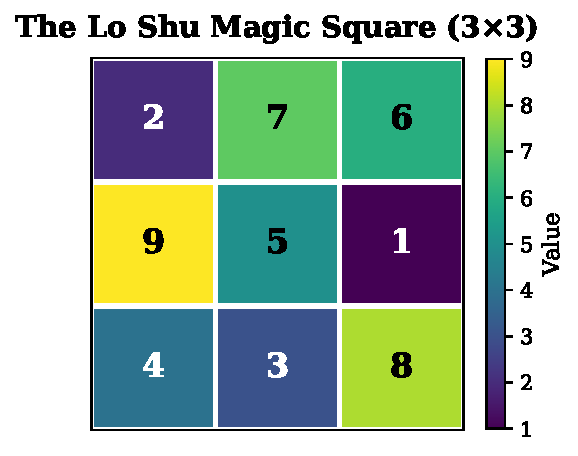
\includegraphics[width=0.4\textwidth]{figures/fig01_lo_shu.pdf}
    \caption{The Lo Shu magic square, the unique (up to symmetry) $3 \times 3$ magic square.
    Each row, column, and diagonal sums to $M(3) = 15$.}
    \label{fig:lo_shu}
\end{figure}

In this paper, we introduce a fundamentally new perspective on magic squares by representing them 
as three-dimensional polyhedra, which we call \emph{Magic Gems}.
The construction arises from a natural physical analogy: imagine placing checkers on an $n \times n$ board,
where the height of each stack corresponds to the number occupying that cell.
This creates a ``topography'' over the grid, and centering this configuration in three-dimensional space
yields a point cloud whose convex hull defines the Magic Gem.

The central insight of this work is that the defining algebraic property of magic squares---equal row, column, and diagonal sums---manifests geometrically as a precise statistical condition.
Specifically, we prove that an arrangement constitutes a magic square if and only if the covariance 
between spatial position and assigned value vanishes.
This zero-covariance theorem provides a bridge between classical combinatorics and multivariate statistics,
offering new tools for understanding and classifying magic squares.

\subsection{Main Contributions}

This paper develops the Magic Gem framework through several interconnected results.
We begin by formalizing the construction of Magic Gems from magic squares
and establishing that symmetry-equivalent squares yield geometrically identical polyhedra,
thus providing a canonical geometric representative for each equivalence class under the dihedral group $D_4$.

Our main theoretical contribution is the Zero-Covariance Theorem (\Cref{thm:zero_covariance}), 
which characterizes magic squares through the vanishing of off-diagonal covariance terms.
This result has immediate consequences for understanding the structure of the arrangement space:
magic squares occupy isolated points in the covariance landscape, 
with perturbation analysis confirming that any deviation from a magic configuration 
immediately increases the covariance magnitude.

We complement these theoretical results with extensive computational experiments on magic squares 
of orders three, four, and five.
These experiments validate our theoretical predictions and reveal the geometric structure 
of both the Magic Gems themselves and the broader space of arrangements in which they reside.
The rarity of magic squares---approximately one in 45,000 random $3 \times 3$ arrangements---corresponds 
to their isolation as zero-covariance configurations in a landscape where generic arrangements 
exhibit substantial covariance.

\subsection{Paper Organization}

The remainder of this paper proceeds as follows.
\Cref{sec:background} reviews classical results on magic squares and establishes notation 
for the geometric and statistical concepts we employ.
\Cref{sec:methodology} presents the Magic Gem construction, proves the Zero-Covariance Theorem,
and develops the perturbation analysis framework.
\Cref{sec:results} describes our computational experiments, validating theoretical predictions 
and exploring the structure of the arrangement space for $n = 3$, $4$, and $5$.
\Cref{sec:discussion} interprets our findings and discusses connections to related areas.
Finally, \Cref{sec:conclusion} summarizes our contributions and outlines directions for future research.

\input{sections/methods}
\section{Computational Results}
\label{sec:results}

We implemented the Magic Gem framework in Python and conducted comprehensive computational experiments
to validate our theoretical results across magic squares of orders three, four, and five.
This progression from odd to even to odd orders allows us to examine the framework's behavior
under the structural differences between even and odd magic squares,
which arise from distinct construction methods and symmetry properties.

\subsection{The 3×3 Case: Foundation and Validation}

The $3 \times 3$ magic square provides the ideal starting point for validating our framework,
as it admits a unique solution (up to symmetry) and allows exhaustive analysis.
The small size of the arrangement space---$9! = 362{,}880$ permutations---permits 
complete enumeration, providing definitive verification of the Zero-Covariance Theorem.

\subsubsection{Exhaustive Verification of the Energy Characterization}

We computed the total magic energy $E(S)$ for all 362,880 permutations of $\{1, \ldots, 9\}$.
This exhaustive analysis confirms the Energy Characterization Theorem (\Cref{thm:energy_char}):
an arrangement has zero energy if and only if it is a magic square.

\Cref{fig:energy_landscape_3x3} displays the energy distribution across all permutations.
The vast majority of arrangements exhibit substantial positive energy,
with the distribution spanning from zero to approximately 20.
Precisely eight configurations---the Lo Shu and its seven $D_4$ symmetry variants---achieve 
$E(S) = 0$ exactly, corresponding to the single essentially different magic square.
No false positives (zero energy but non-magic) or false negatives (magic but nonzero energy) exist,
providing complete verification of the theorem for $n = 3$.

\begin{figure}[H]
    \centering
    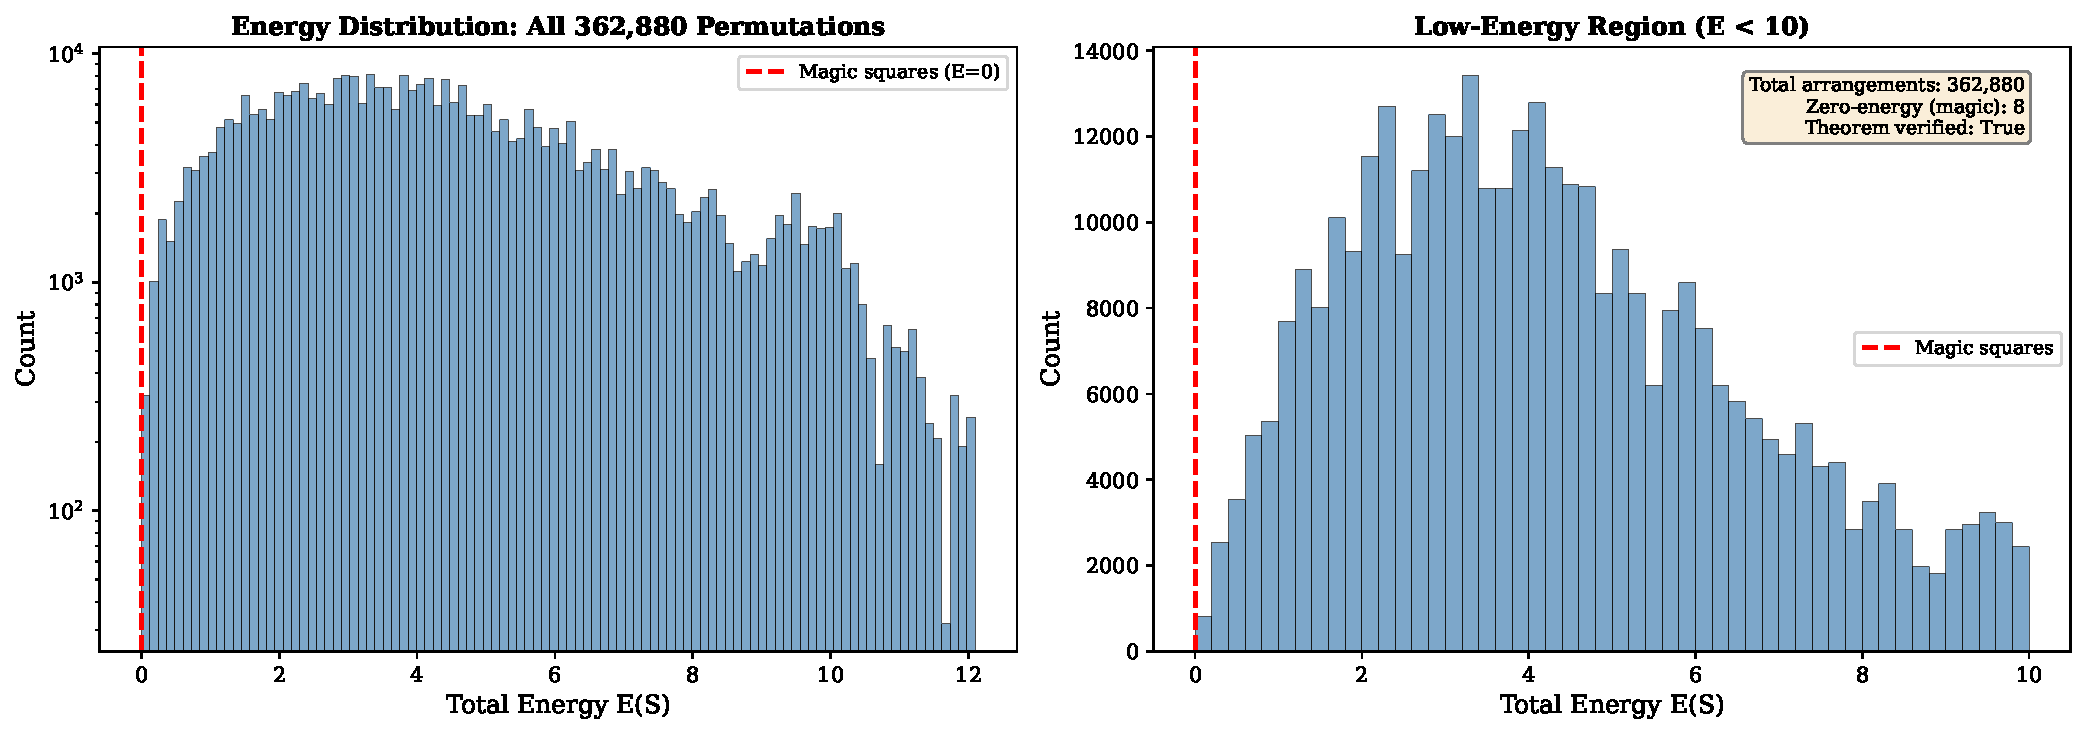
\includegraphics[width=0.95\textwidth]{figures/fig21_energy_landscape_n3.pdf}
    \caption{Energy landscape for $n = 3$. Left: Distribution of total energy across all 362,880 permutations (log scale). 
    The eight magic squares occupy the unique zero-energy position. 
    Right: Zoomed view of the low-energy region, showing the gap between magic squares and all other arrangements.}
    \label{fig:energy_landscape_3x3}
\end{figure}

The energy landscape reveals the exceptional nature of magic squares.
While generic permutations cluster around a mean energy of approximately 2.5,
magic squares are isolated at the absolute minimum.
The gap between zero and the smallest positive energy provides a quantitative measure 
of the ``stability'' of the magic property.

\subsubsection{Perturbation Isolation Analysis}

To verify that magic squares are strict local minima, we analyzed the effect of single-swap perturbations.
For each of the eight magic squares, we computed the energy after every possible swap 
of two elements, yielding $\binom{9}{2} = 36$ perturbed arrangements per square.

\Cref{fig:perturbation_gaps} shows the distribution of minimum energy gaps.
Every single swap increases the energy, with a minimum gap of approximately 0.02 across all magic squares.
This confirms that magic squares are isolated in the energy landscape:
there is no continuous path of decreasing energy leading away from a magic configuration.
The physical interpretation is compelling---magic squares sit at the bottom of steep-walled wells,
and any perturbation immediately rolls the configuration uphill.

\begin{figure}[H]
    \centering
    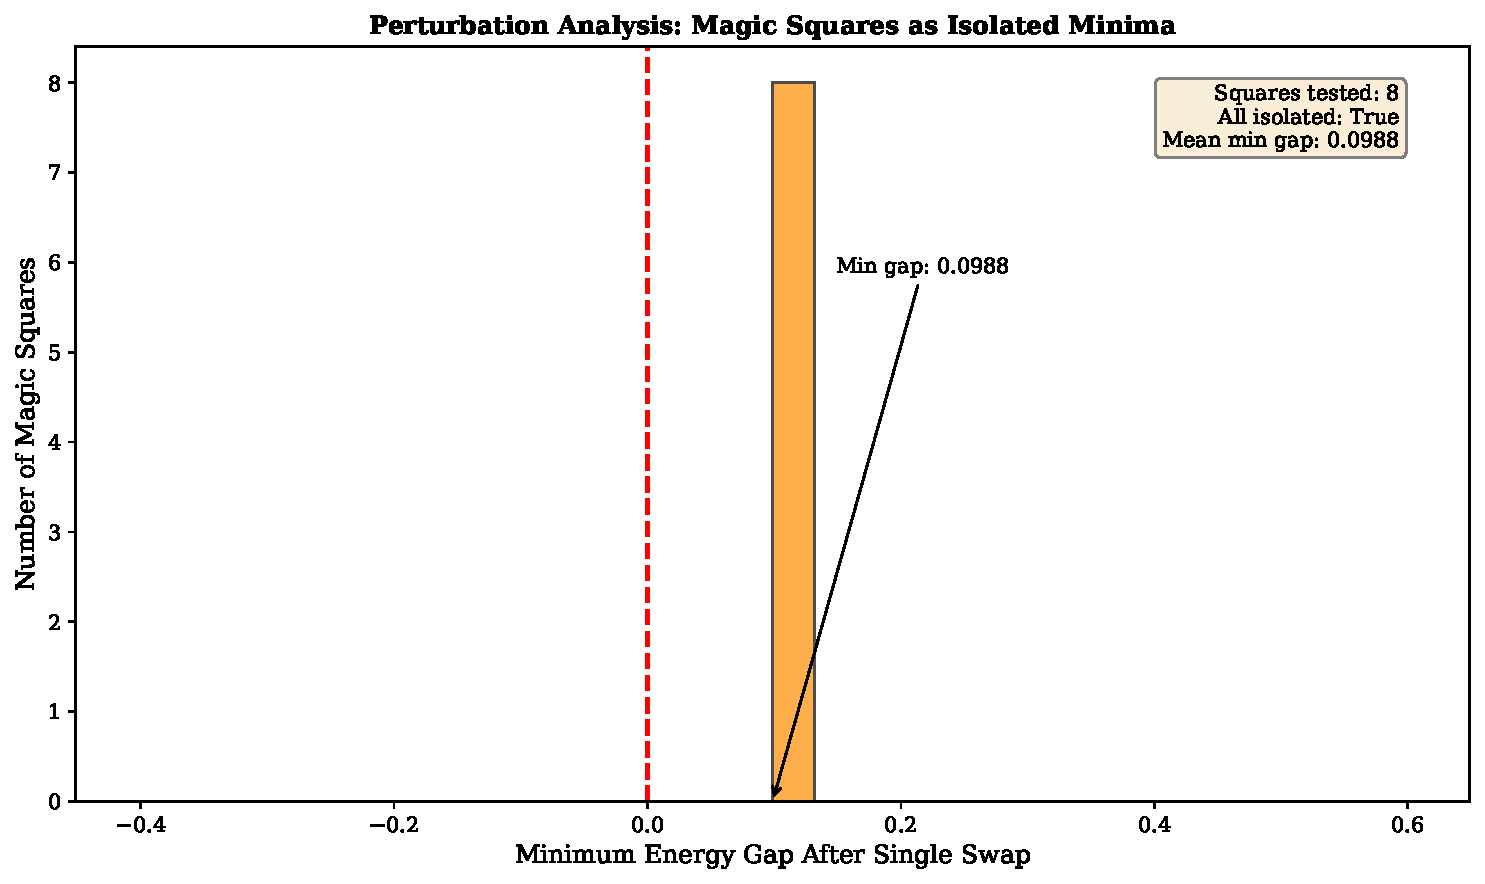
\includegraphics[width=0.7\textwidth]{figures/fig22_perturbation_gaps.pdf}
    \caption{Perturbation analysis showing minimum energy gap after single-swap perturbations.
    All eight magic squares are isolated local minima, with every swap increasing energy.}
    \label{fig:perturbation_gaps}
\end{figure}

\subsubsection{Zero-Covariance Verification}

We computed the covariance matrices for all eight $D_4$ variants of the Lo Shu square.
As predicted by \Cref{thm:zero_covariance}, every variant achieves
$\Cov(X, Z) = \Cov(Y, Z) = 0$ to machine precision.
To contextualize this result, we generated 10,000 random arrangements 
by permuting the integers 1 through 9 and computed covariances for each.

\Cref{fig:covariance_3x3} displays the resulting distributions.
The covariances for random arrangements spread broadly around zero,
with standard deviation approximately 0.84.
While the distributions are centered near zero (as expected from symmetry),
achieving exactly zero is exceptionally rare:
only 8 of the 362,880 possible arrangements are magic, a proportion of roughly 0.002\%.

\begin{figure}[H]
    \centering
    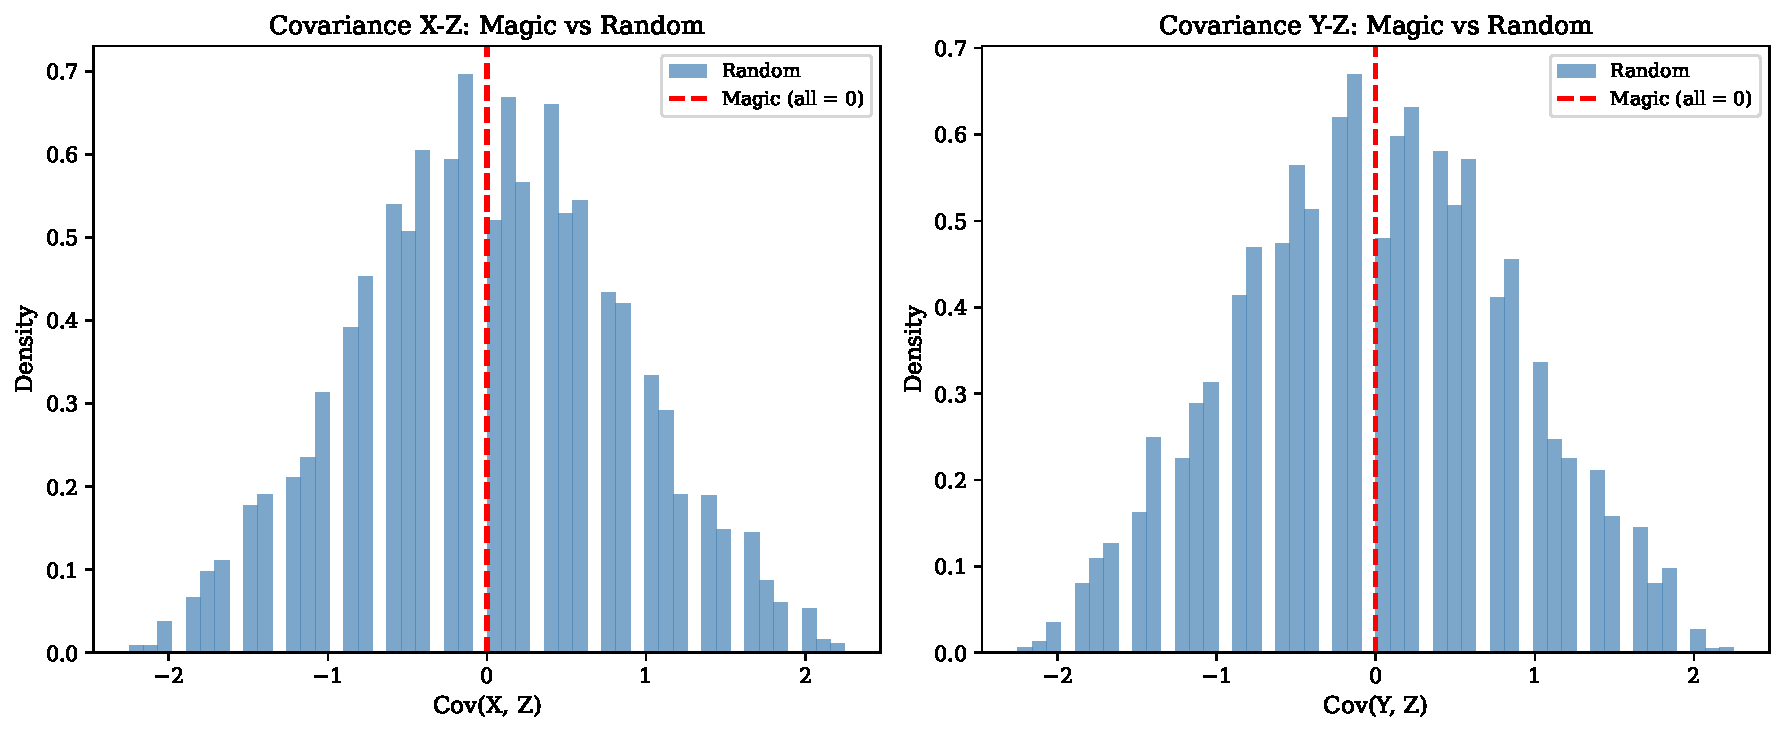
\includegraphics[width=0.9\textwidth]{figures/fig06_covariance_3x3.pdf}
    \caption{Covariance distributions for 5,000 random $3 \times 3$ arrangements.
    The magic square value of exactly zero (red dashed line) lies at the center
    but is achieved by only 8 of 362,880 possible arrangements.}
    \label{fig:covariance_3x3}
\end{figure}

\subsubsection{Geometric Structure}

The $3 \times 3$ Magic Gem comprises nine points, of which eight lie on the convex hull
while the ninth---corresponding to the center cell with value 5---occupies the interior at the origin.
\Cref{fig:magic_gem_3x3} visualizes this structure, with the hull rendered as translucent faces
and vertices colored by their $z$-values.

\begin{figure}[H]
    \centering
    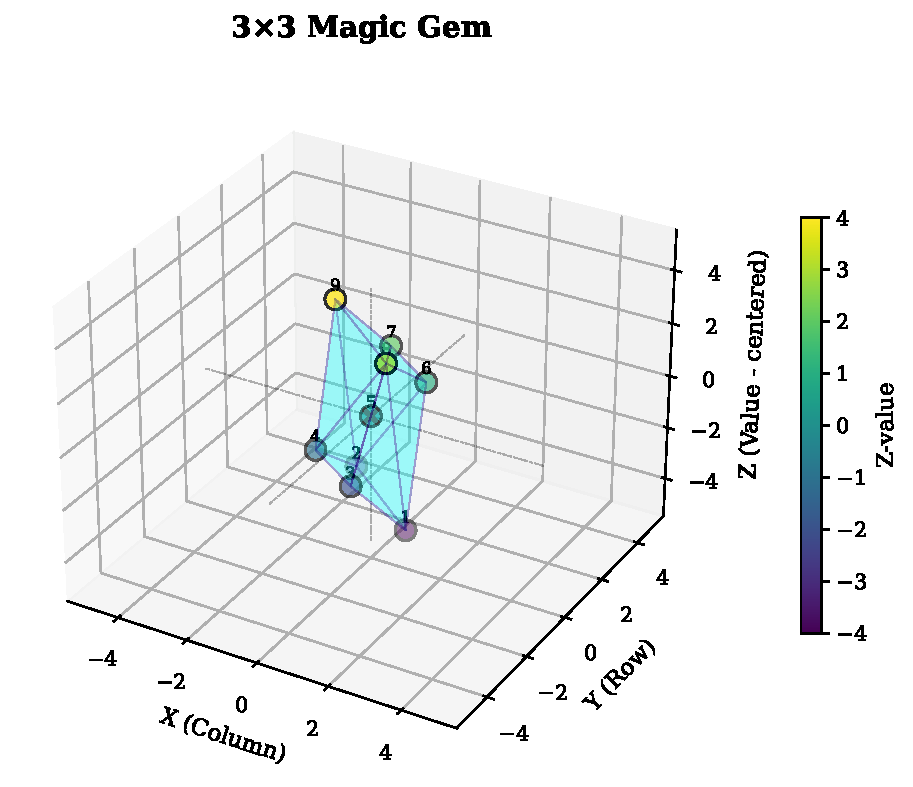
\includegraphics[width=0.7\textwidth]{figures/fig03_magic_gem_3x3.pdf}
    \caption{The $3 \times 3$ Magic Gem showing vertex positions colored by $z$-value
    and the convex hull with translucent faces.
    The center point lies at the origin, interior to the hull.}
    \label{fig:magic_gem_3x3}
\end{figure}

The vector representation, shown in \Cref{fig:vectors_3x3}, displays all nine vectors from the centroid.
The balanced distribution---vectors in each direction having $z$-components 
that sum to zero when weighted by position---visually manifests the zero-covariance property.

\begin{figure}[H]
    \centering
    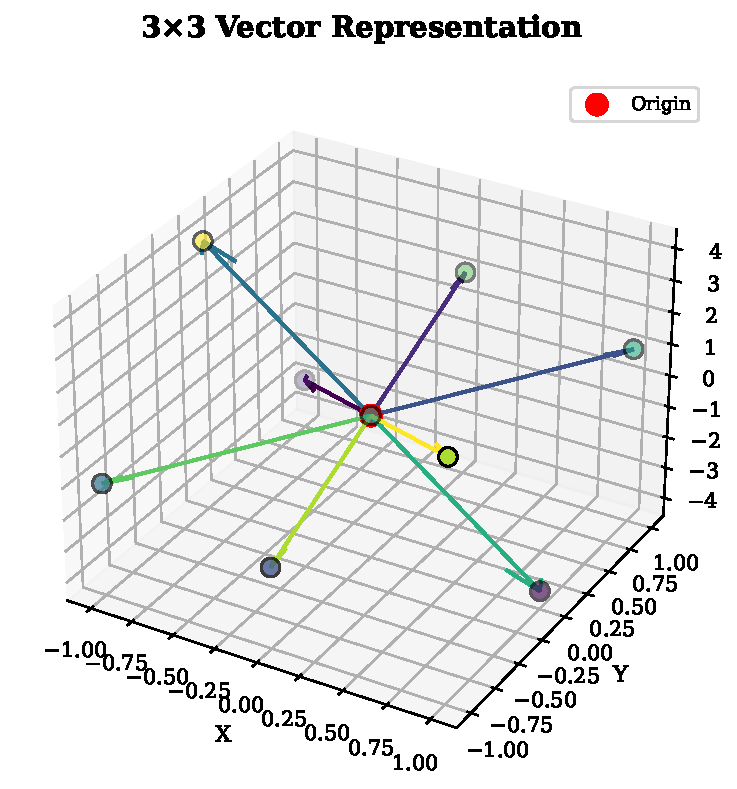
\includegraphics[width=0.7\textwidth]{figures/fig04_vectors_3x3.pdf}
    \caption{Vector representation of the $3 \times 3$ Magic Gem,
    showing nine vectors from the centroid to each vertex.}
    \label{fig:vectors_3x3}
\end{figure}

The hull volume distribution (\Cref{fig:hull_volume_3x3}) places the Magic Gem's volume 
of 18 cubic units near the center of the distribution for random arrangements,
indicating that magic squares are distinguished by their covariance structure
rather than geometric extremality.

\begin{figure}[H]
    \centering
    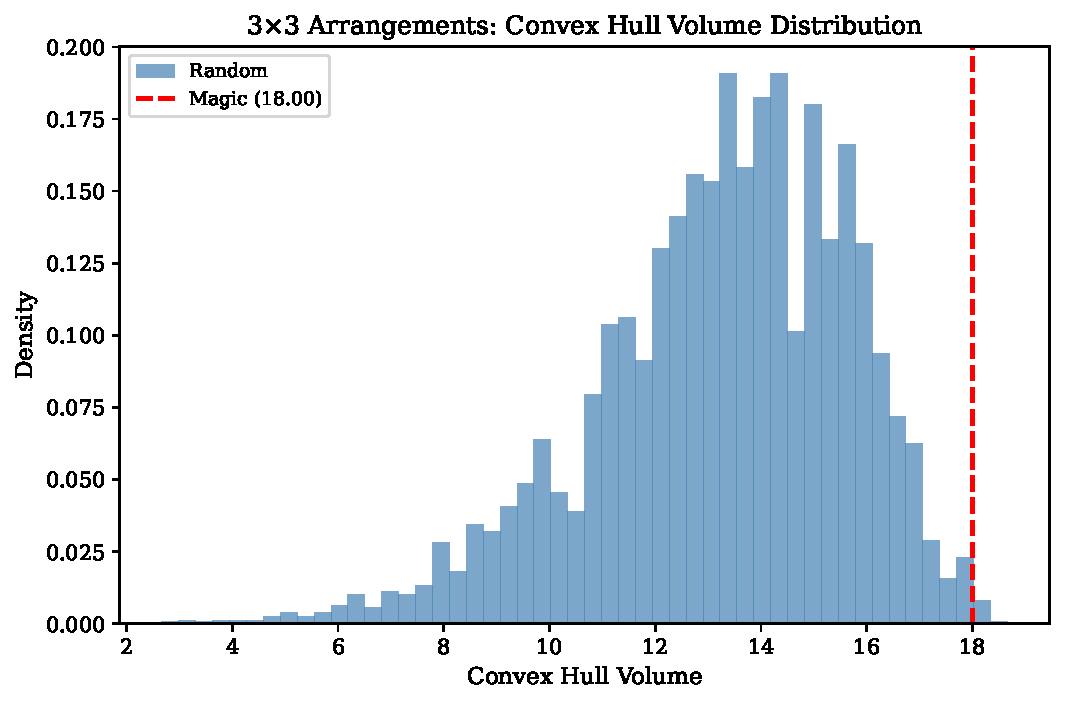
\includegraphics[width=0.7\textwidth]{figures/fig07_hull_volume_3x3.pdf}
    \caption{Convex hull volume distribution for 5,000 random $3 \times 3$ arrangements.
    The Magic Gem volume (red line) lies near the distribution center.}
    \label{fig:hull_volume_3x3}
\end{figure}

\subsection{The 4×4 Case: Even-Order Analysis}

The transition to $n = 4$ introduces several important changes.
First, $4 \times 4$ magic squares require different construction methods than odd orders---the 
doubly-even method replaces the Siamese method.
Second, there exist 880 essentially different $4 \times 4$ magic squares,
providing a richer landscape for geometric study.
Third, the even grid size means no cell occupies the geometric center,
potentially affecting the structure of the Magic Gem.

\subsubsection{Construction and Visualization}

\Cref{fig:magic_square_4x4} shows the $4 \times 4$ magic square constructed via the doubly-even method,
with magic constant $M(4) = 34$.
The construction process, illustrated in \Cref{fig:construction_4x4}, 
follows the same four steps as for odd orders:
grid centering, $z$-value assignment, centering of $z$-values, and hull computation.

\begin{figure}[H]
    \centering
    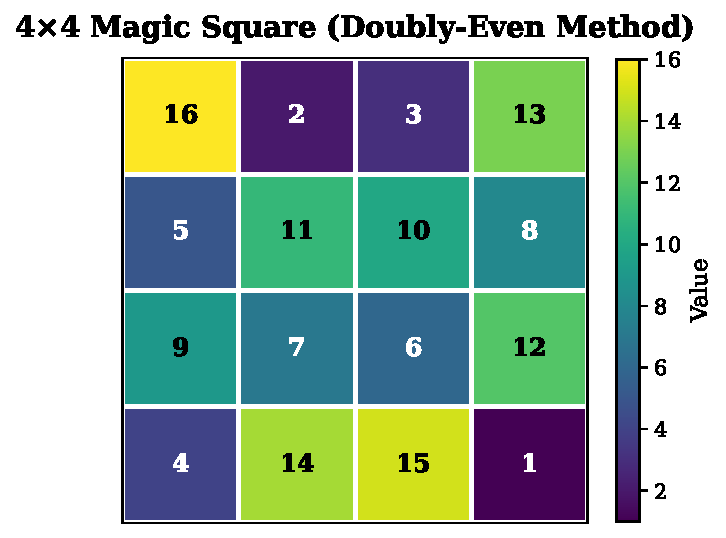
\includegraphics[width=0.45\textwidth]{figures/fig08_magic_square_4x4.pdf}
    \caption{A $4 \times 4$ magic square constructed via the doubly-even method.
    Each row, column, and diagonal sums to $M(4) = 34$.}
    \label{fig:magic_square_4x4}
\end{figure}

\begin{figure}[H]
    \centering
    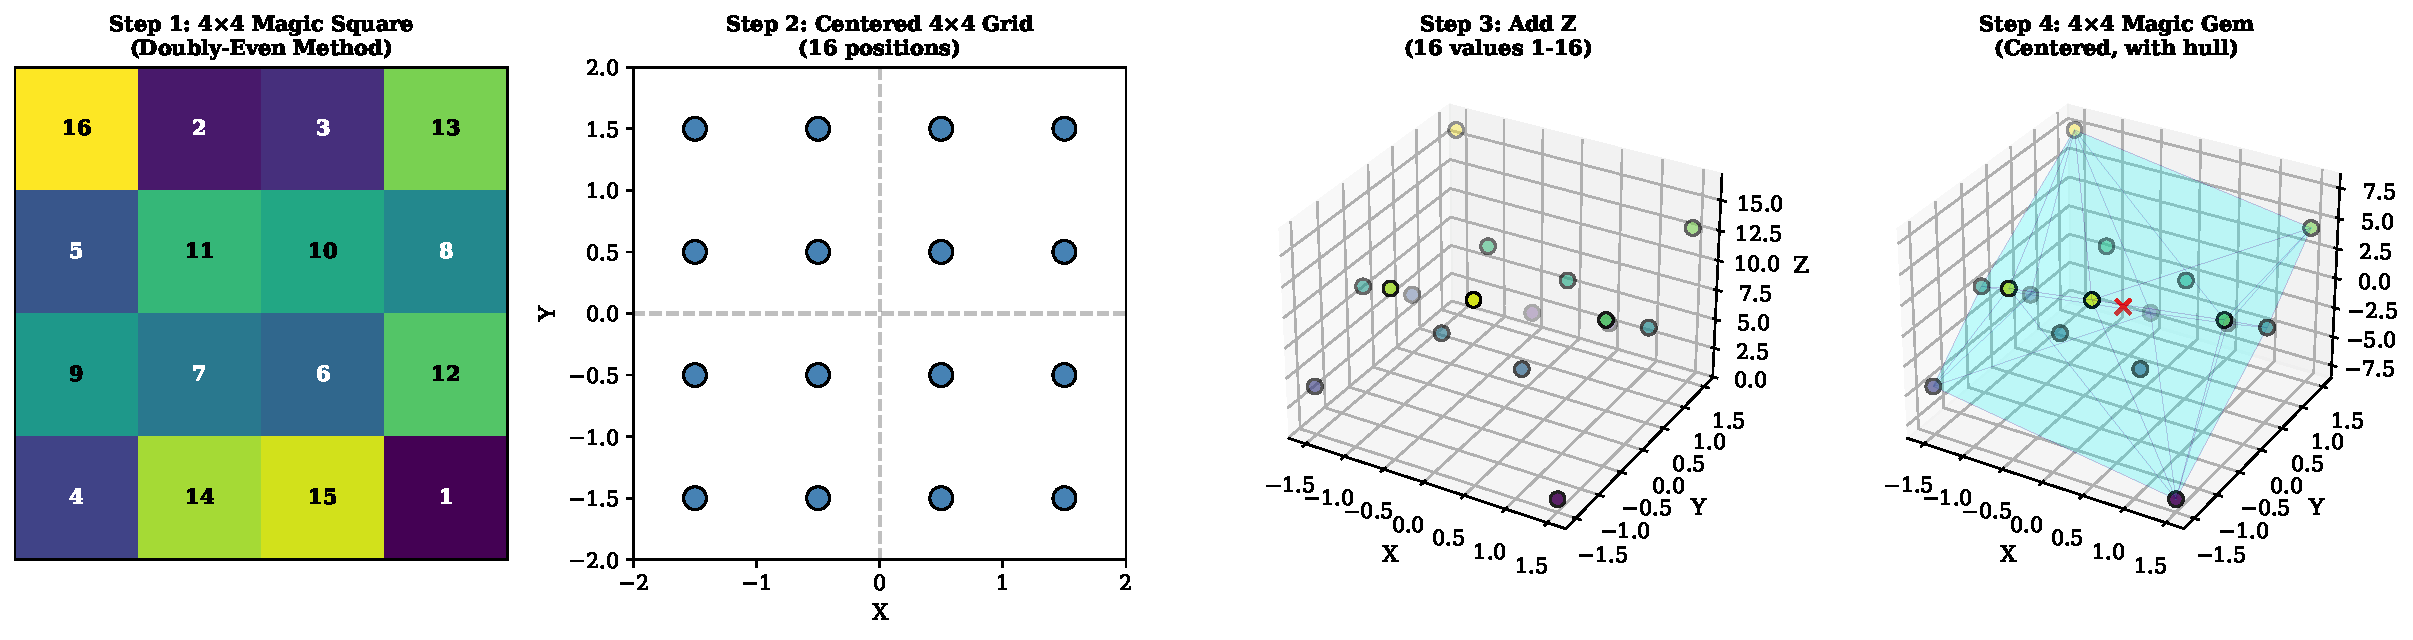
\includegraphics[width=\textwidth]{figures/fig09_construction_4x4.pdf}
    \caption{Construction of the $4 \times 4$ Magic Gem, showing the four-step process
    from magic square to centered polyhedral representation.}
    \label{fig:construction_4x4}
\end{figure}

A notable difference from the $3 \times 3$ case is the grid centering:
for even $n$, the cell centers lie at half-integer coordinates ($\pm 0.5, \pm 1.5$),
and no cell coincides with the origin.
Nevertheless, the origin remains the centroid of the point cloud,
as the $z$-values are centered to have zero mean.

\subsubsection{Zero-Covariance for Even Order}

The Zero-Covariance Theorem makes no distinction between even and odd orders,
predicting $\Cov(X, Z) = \Cov(Y, Z) = 0$ for all magic squares.
Our computations confirm this prediction for the $4 \times 4$ case:
the magic square achieves exactly zero covariance to machine precision.

\Cref{fig:covariance_4x4} compares the magic covariance to 3,000 random $4 \times 4$ arrangements.
The distributions are somewhat narrower than for $3 \times 3$ (relative to their range),
reflecting the increased constraints imposed by having 16 cells rather than 9.
The magic square again sits precisely at zero.

\begin{figure}[H]
    \centering
    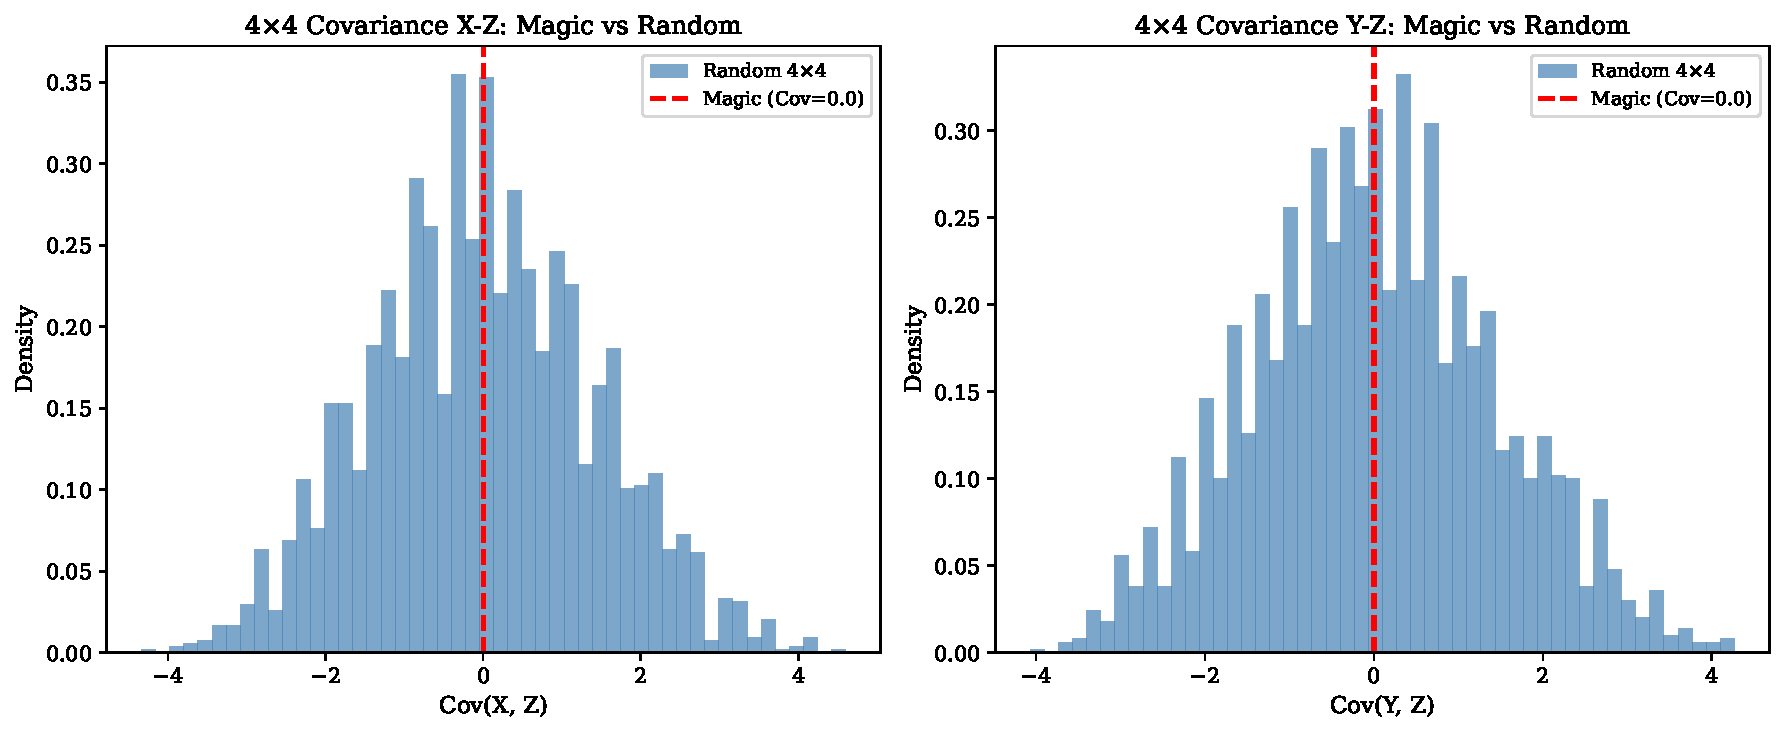
\includegraphics[width=0.9\textwidth]{figures/fig12_covariance_4x4.pdf}
    \caption{Covariance distributions for 3,000 random $4 \times 4$ arrangements,
    with the magic square value of exactly zero marked.}
    \label{fig:covariance_4x4}
\end{figure}

\subsubsection{Geometric Properties}

The $4 \times 4$ Magic Gem, shown in \Cref{fig:magic_gem_4x4}, has 16 vertices.
Unlike the $3 \times 3$ case where only one point (the center) is interior,
the $4 \times 4$ gem has multiple interior points, with approximately 12 vertices on the hull.

\begin{figure}[H]
    \centering
    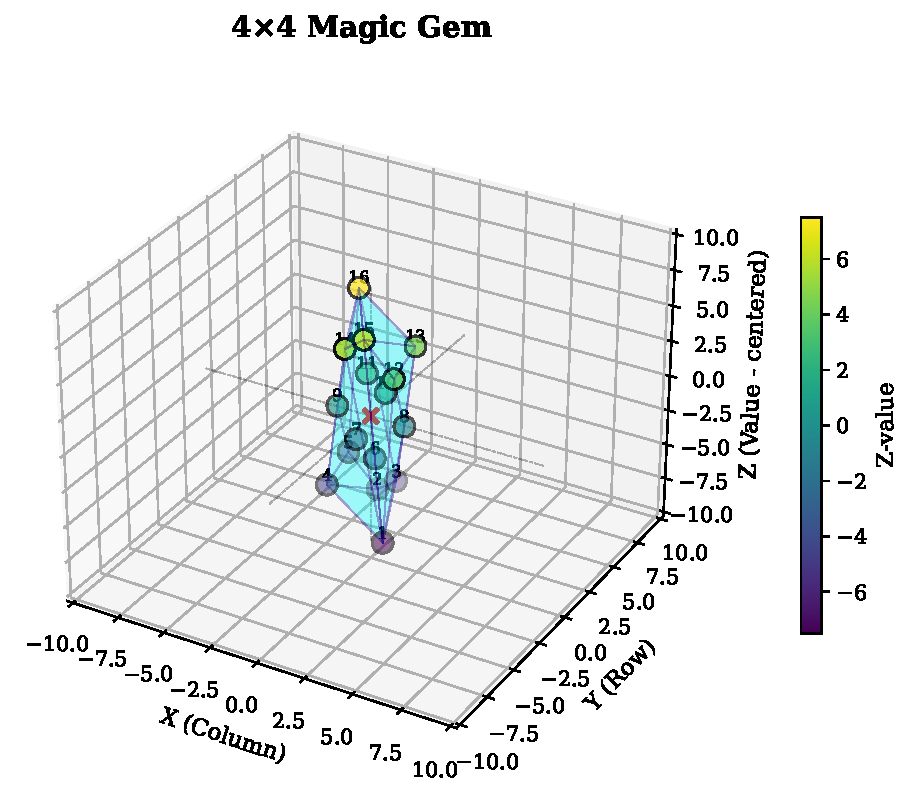
\includegraphics[width=0.7\textwidth]{figures/fig10_magic_gem_4x4.pdf}
    \caption{The $4 \times 4$ Magic Gem showing 16 vertices colored by $z$-value.
    The more complex structure reflects the larger grid size.}
    \label{fig:magic_gem_4x4}
\end{figure}

The vector representation (\Cref{fig:vectors_4x4}) displays 16 vectors from the centroid.
Despite the absence of a central cell, the vectors remain balanced according to the zero-covariance criterion.

\begin{figure}[H]
    \centering
    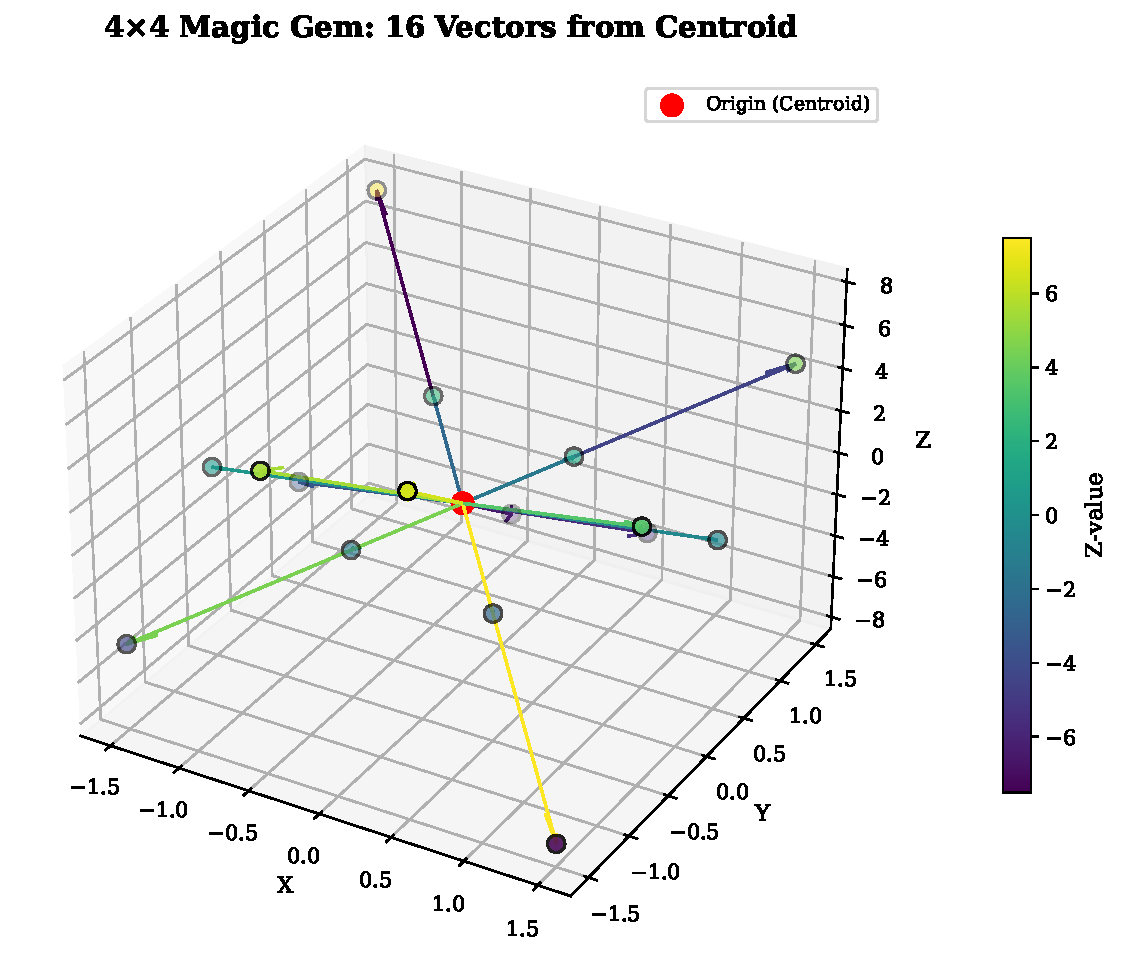
\includegraphics[width=0.7\textwidth]{figures/fig11_vectors_4x4.pdf}
    \caption{Vector representation of the $4 \times 4$ Magic Gem,
    showing 16 vectors from the centroid.}
    \label{fig:vectors_4x4}
\end{figure}

\Cref{fig:hull_volume_4x4} shows the hull volume distribution for random $4 \times 4$ arrangements.
As with the $3 \times 3$ case, the Magic Gem volume falls near the center of the distribution.

\begin{figure}[H]
    \centering
    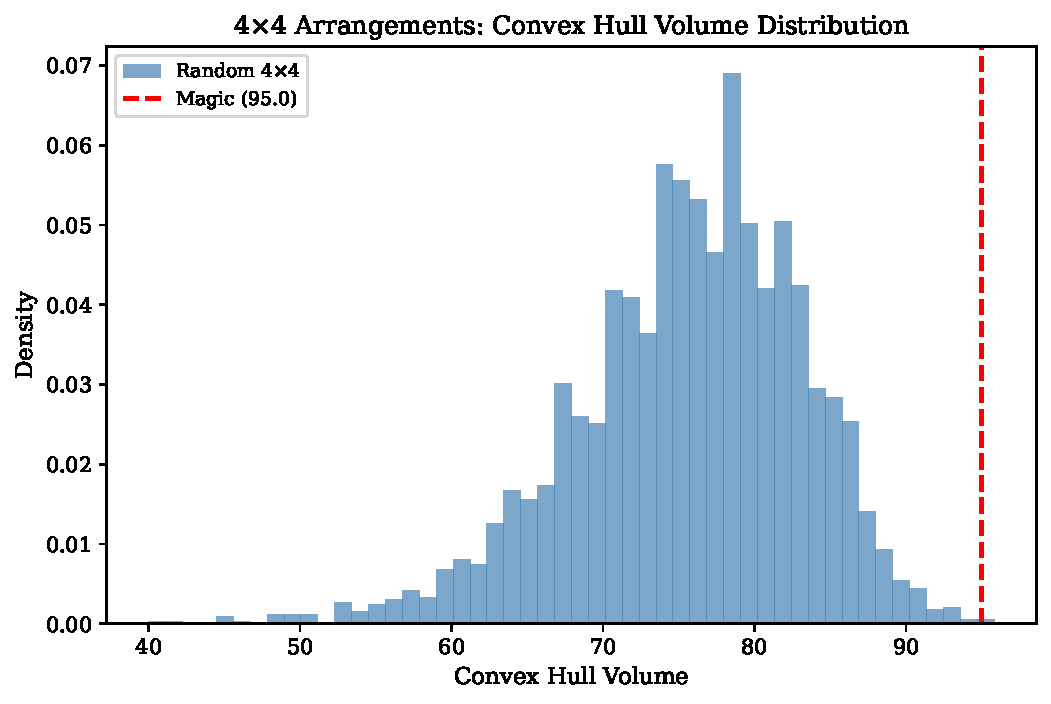
\includegraphics[width=0.7\textwidth]{figures/fig13_hull_volume_4x4.pdf}
    \caption{Convex hull volume distribution for 3,000 random $4 \times 4$ arrangements.}
    \label{fig:hull_volume_4x4}
\end{figure}

\subsection{The 5×5 Case: Return to Odd Order}

Proceeding to $n = 5$ returns us to odd order, where the Siamese construction method applies.
The $5 \times 5$ case is substantially more complex:
there exist approximately 275 million magic squares forming about 34 million equivalence classes.

\subsubsection{Construction and Visualization}

\Cref{fig:magic_square_5x5} shows the $5 \times 5$ magic square with magic constant $M(5) = 65$.
The Siamese method produces a characteristic diagonal pattern visible in the arrangement.

\begin{figure}[H]
    \centering
    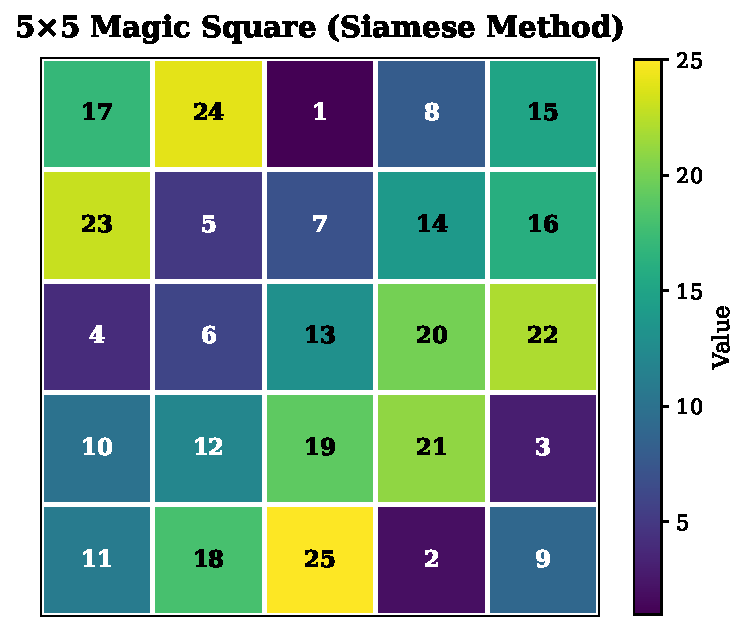
\includegraphics[width=0.5\textwidth]{figures/fig14_magic_square_5x5.pdf}
    \caption{A $5 \times 5$ magic square constructed via the Siamese method.
    Each row, column, and diagonal sums to $M(5) = 65$.}
    \label{fig:magic_square_5x5}
\end{figure}

The construction process (\Cref{fig:construction_5x5}) maps the 25-cell grid 
to 25 points in $\R^3$, with the central cell again coinciding with the origin.

\begin{figure}[H]
    \centering
    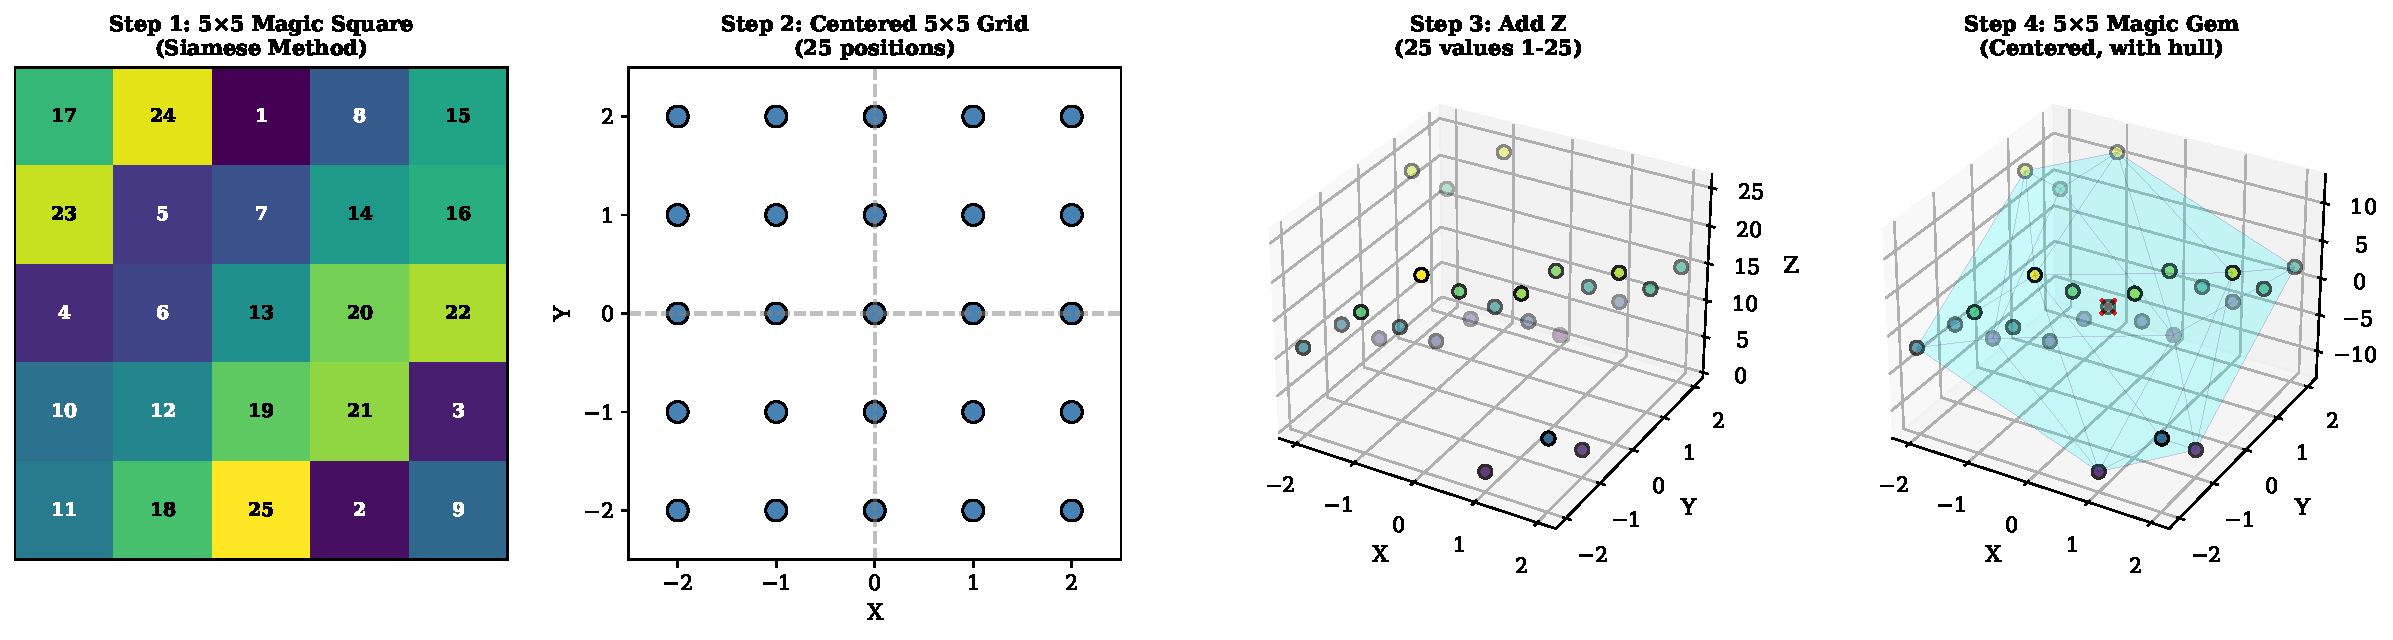
\includegraphics[width=\textwidth]{figures/fig15_construction_5x5.pdf}
    \caption{Construction of the $5 \times 5$ Magic Gem.}
    \label{fig:construction_5x5}
\end{figure}

\subsubsection{Zero-Covariance Verification}

The $5 \times 5$ magic square achieves $\Cov(X, Z) = \Cov(Y, Z) = 0$ exactly,
as predicted by the theorem.
\Cref{fig:covariance_5x5} compares this to 3,000 random arrangements.
The covariance distributions are wider than for smaller orders
(reflecting the larger range of values 1--25),
but the magic square remains precisely at zero.

\begin{figure}[H]
    \centering
    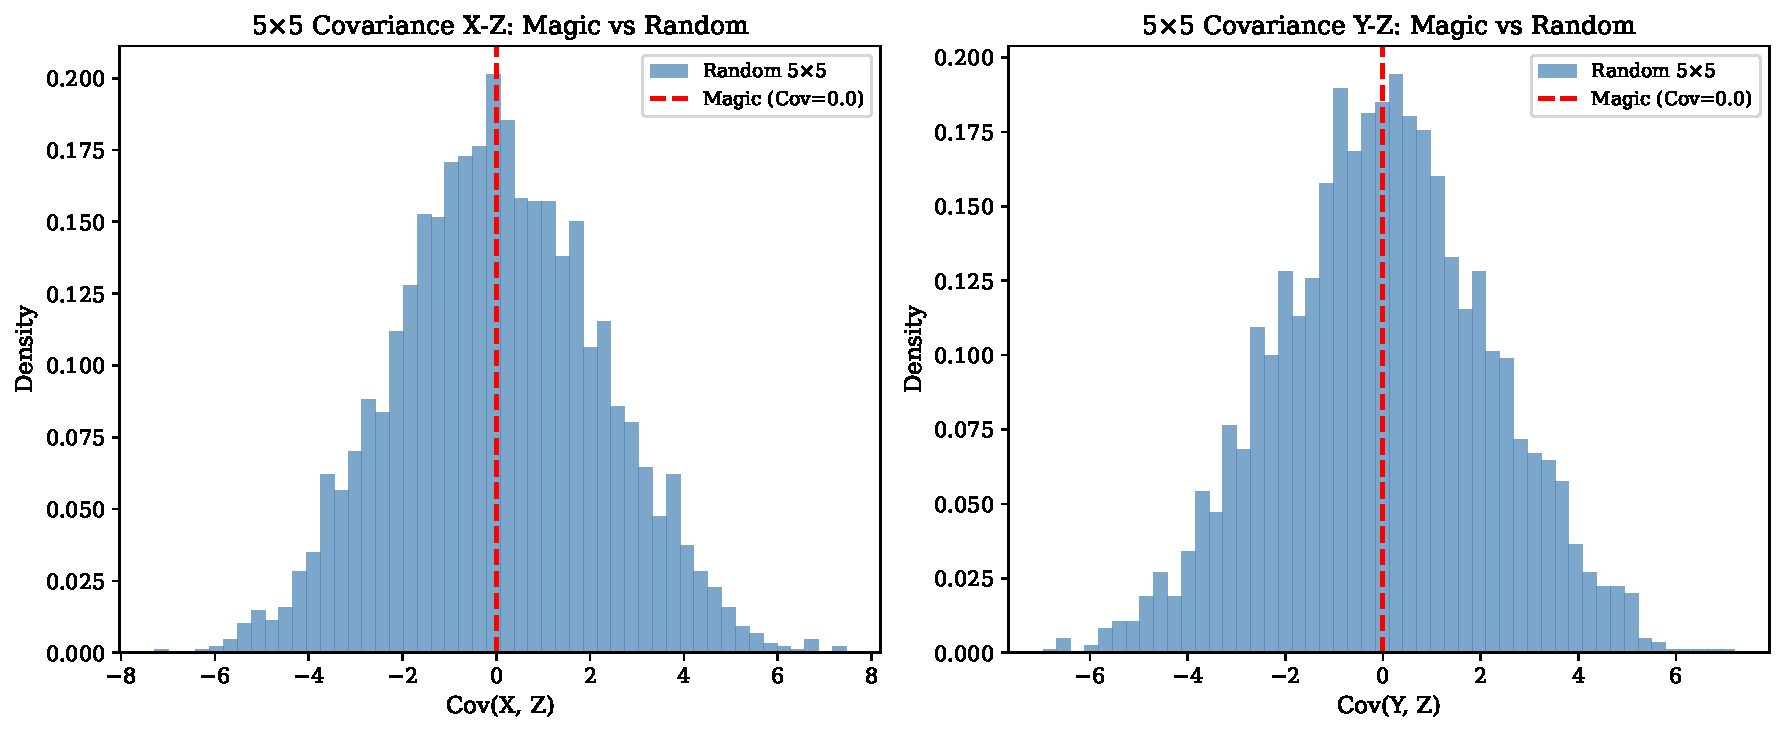
\includegraphics[width=0.9\textwidth]{figures/fig18_covariance_5x5.pdf}
    \caption{Covariance distributions for 3,000 random $5 \times 5$ arrangements.
    The wider spread reflects the larger value range, but magic squares still achieve exactly zero.}
    \label{fig:covariance_5x5}
\end{figure}

\subsubsection{Geometric Properties}

The $5 \times 5$ Magic Gem (\Cref{fig:magic_gem_5x5}) exhibits substantially greater complexity.
Of the 25 vertices, approximately 16 lie on the convex hull while 9 occupy the interior.
The vector representation (\Cref{fig:vectors_5x5}) shows the balanced distribution of 25 vectors.

\begin{figure}[H]
    \centering
    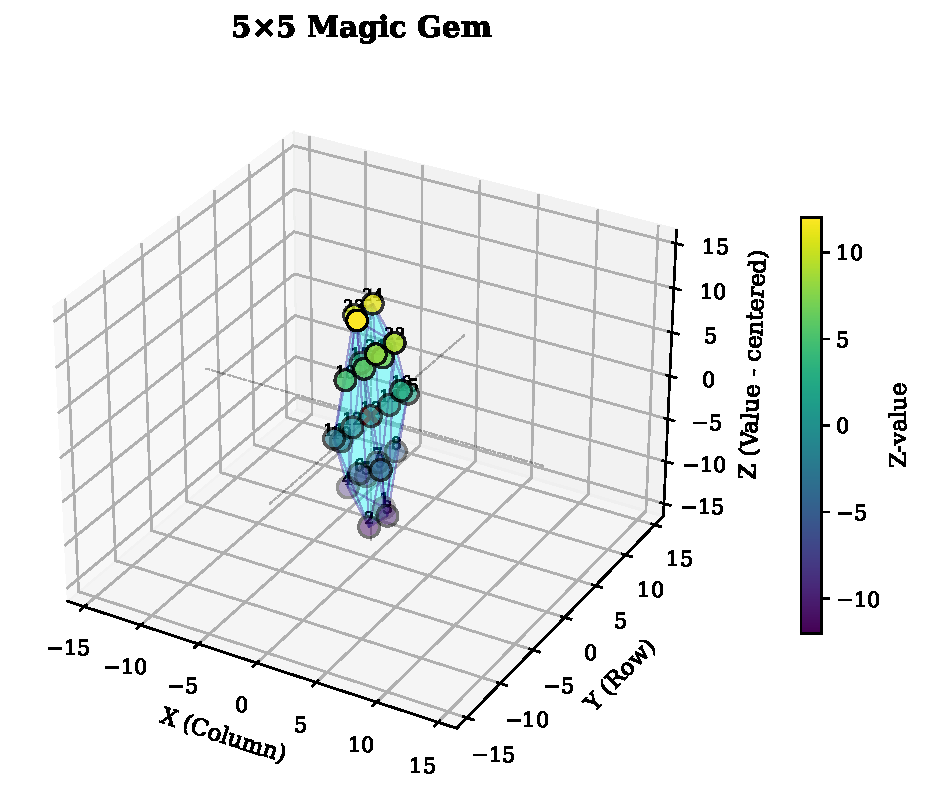
\includegraphics[width=0.7\textwidth]{figures/fig16_magic_gem_5x5.pdf}
    \caption{The $5 \times 5$ Magic Gem showing 25 vertices and the convex hull.}
    \label{fig:magic_gem_5x5}
\end{figure}

\begin{figure}[H]
    \centering
    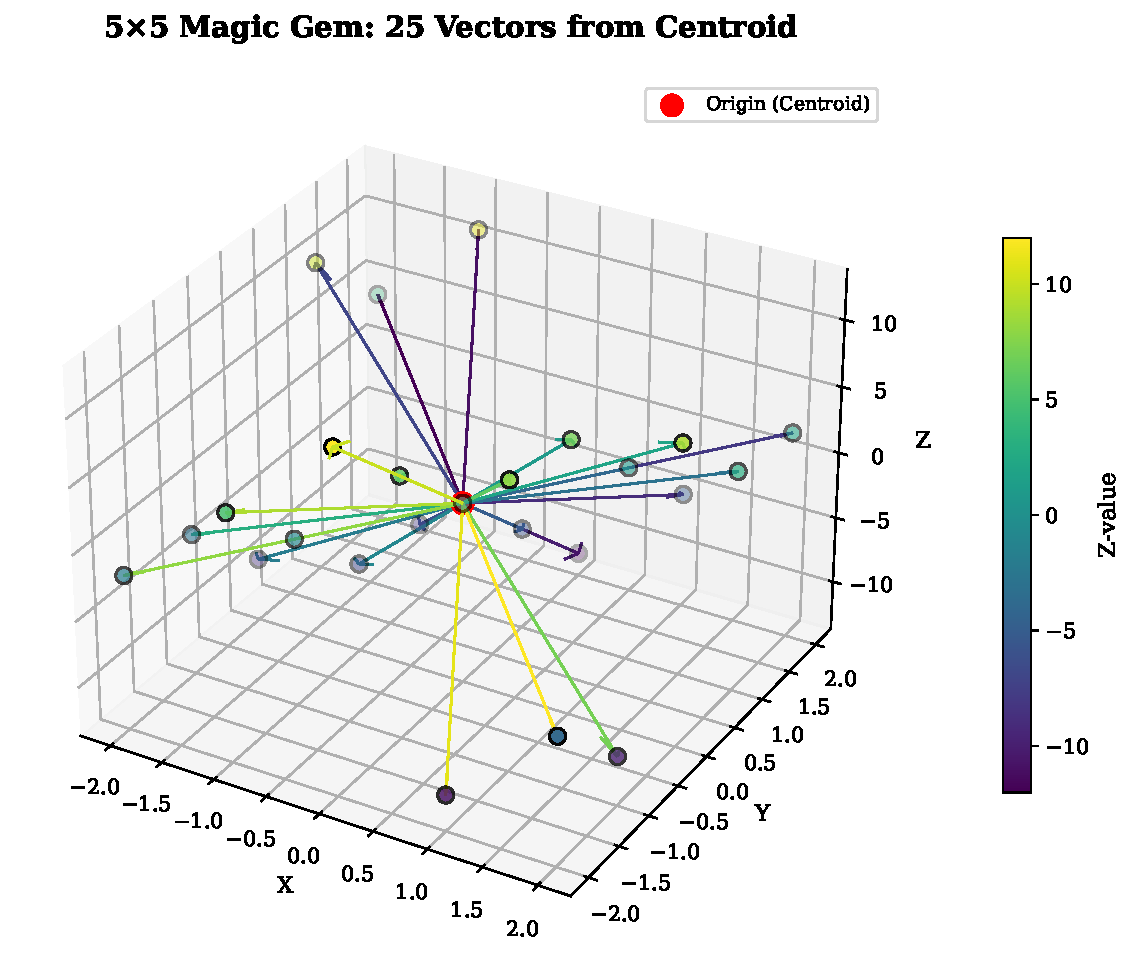
\includegraphics[width=0.7\textwidth]{figures/fig17_vectors_5x5.pdf}
    \caption{Vector representation of the $5 \times 5$ Magic Gem.}
    \label{fig:vectors_5x5}
\end{figure}

\begin{figure}[H]
    \centering
    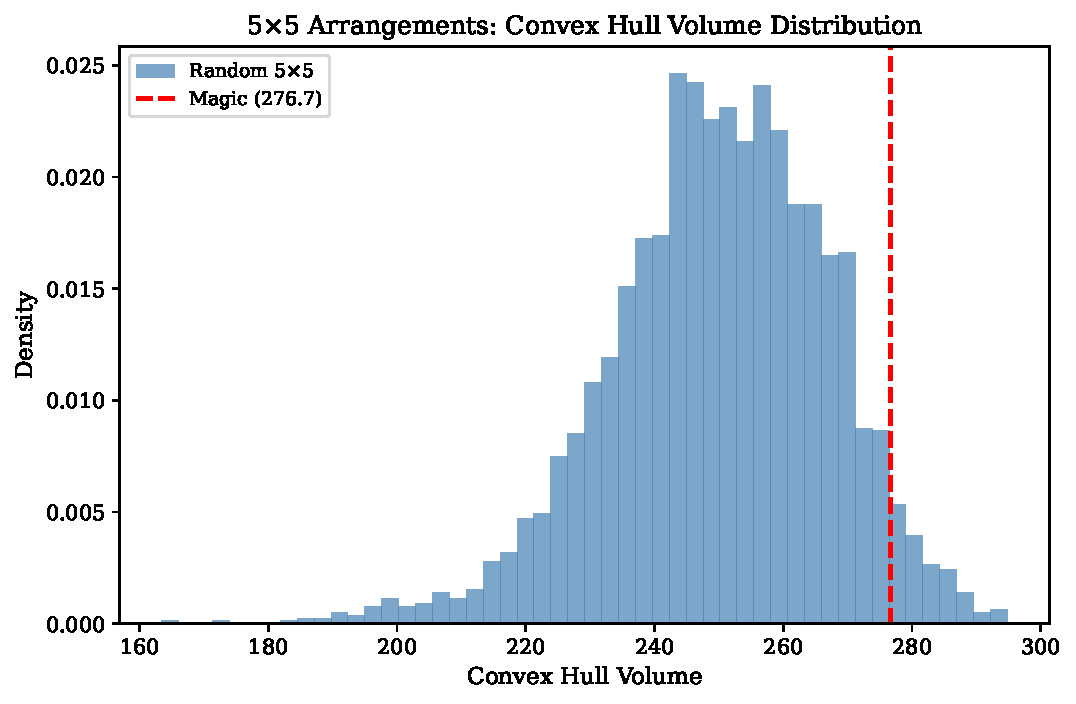
\includegraphics[width=0.7\textwidth]{figures/fig19_hull_volume_5x5.pdf}
    \caption{Convex hull volume distribution for 3,000 random $5 \times 5$ arrangements.}
    \label{fig:hull_volume_5x5}
\end{figure}

\subsection{Scaling Analysis Across Orders}

\Cref{fig:scaling_analysis} presents a systematic comparison of geometric and energy properties 
across orders $n = 3, 4, 5$, revealing how the structure of Magic Gems evolves with increasing complexity.

\begin{figure}[H]
    \centering
    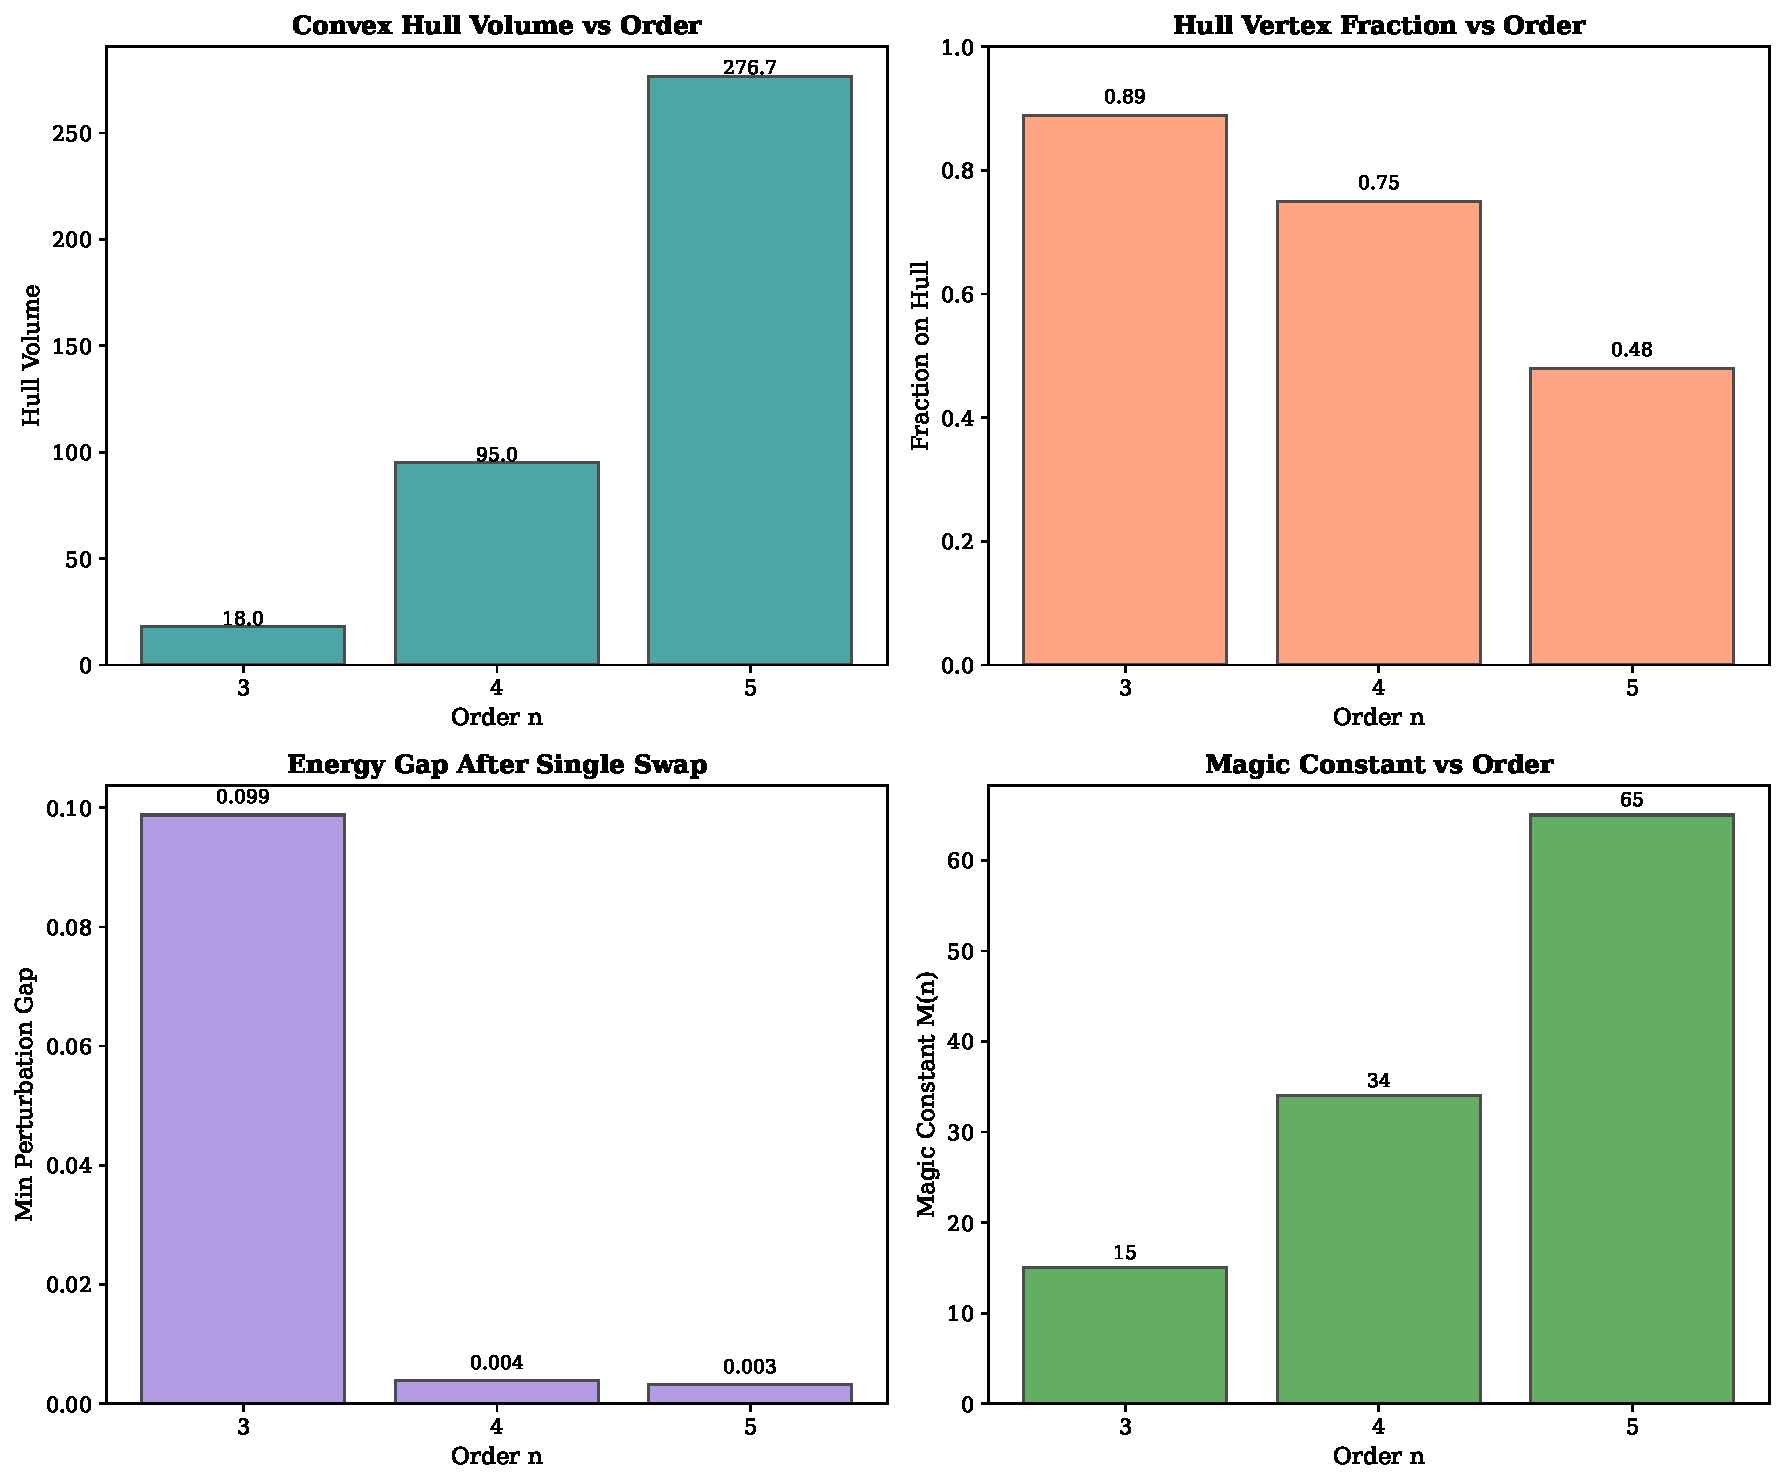
\includegraphics[width=0.95\textwidth]{figures/fig23_scaling_analysis.pdf}
    \caption{Scaling analysis across orders $n = 3, 4, 5$. 
    (a) Convex hull volume increases with order, reflecting the larger range of $z$-values.
    (b) The fraction of points on the hull boundary decreases as interior points proliferate.
    (c) The minimum perturbation gap decreases with order, suggesting larger magic squares 
    are ``less isolated'' in the energy landscape.
    (d) The magic constant $M(n) = n(n^2+1)/2$ grows quadratically.}
    \label{fig:scaling_analysis}
\end{figure}

Several patterns emerge from this analysis.
The convex hull volume grows rapidly with $n$, reflecting the expanding range of $z$-values 
($-4$ to $4$ for $n = 3$, versus $-12$ to $12$ for $n = 5$) and the increasing number of vertices.
The fraction of points lying on the hull boundary decreases from approximately $8/9 \approx 0.89$ for $n = 3$ 
to roughly $0.64$ for $n = 5$, as the interior of the hull becomes more populated.

Perhaps most intriguingly, the minimum perturbation gap---the smallest energy increase 
resulting from any single swap---decreases with order.
For $n = 3$, the gap is approximately 0.02; for $n = 5$, it drops to roughly 0.006.
This suggests that larger magic squares are ``less isolated'' in the energy landscape,
sitting in shallower wells with walls that rise more gradually.
Whether this trend continues for larger $n$ remains an open question,
with implications for the difficulty of constructing or recognizing magic squares of high order.

\subsection{Cross-Order Comparison}

\Cref{fig:comparison_all} provides a unified view of Magic Gems across all three orders,
highlighting the progression in complexity while maintaining the invariant zero-covariance property.

\begin{figure}[H]
    \centering
    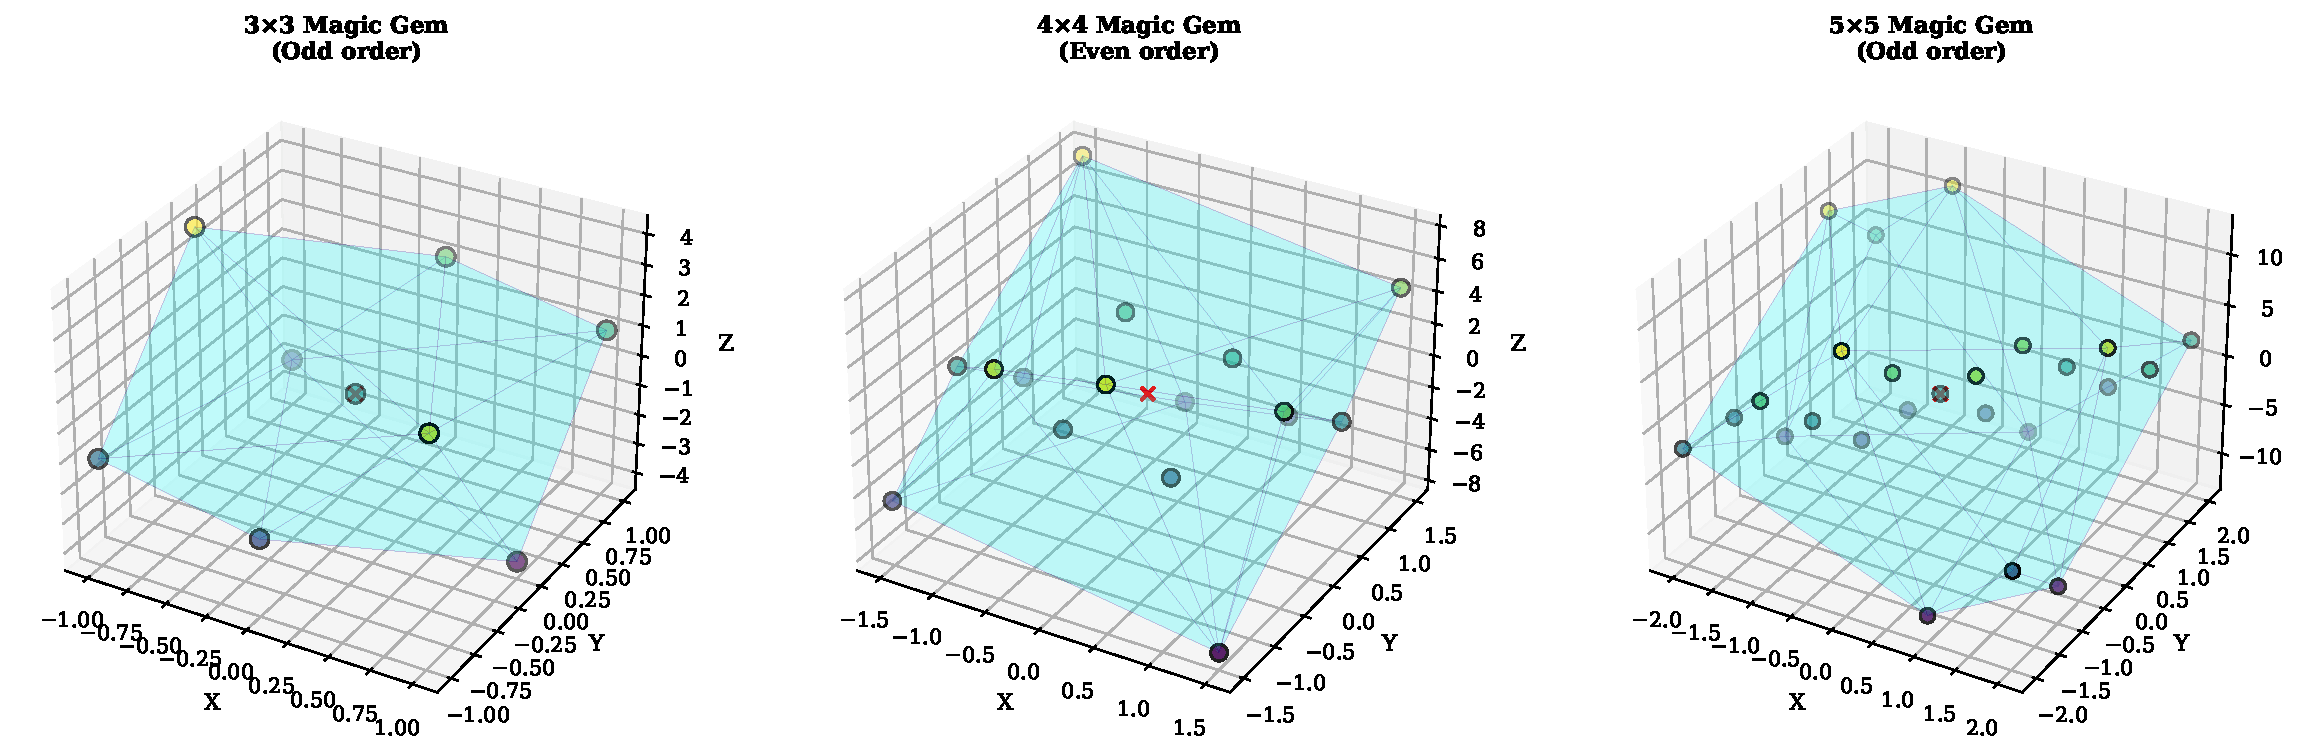
\includegraphics[width=\textwidth]{figures/fig20_comparison_all_orders.pdf}
    \caption{Side-by-side comparison of $3 \times 3$, $4 \times 4$, and $5 \times 5$ Magic Gems.
    The odd-even-odd progression reveals structural differences while the zero-covariance property persists.}
    \label{fig:comparison_all}
\end{figure}

\Cref{tab:comparison_all} summarizes key properties across orders,
demonstrating both the growth in complexity and the invariance of the zero-covariance characterization.

\begin{table}[H]
\centering
\begin{tabular}{lccc}
\toprule
Property & $n = 3$ & $n = 4$ & $n = 5$ \\
\midrule
Order parity & Odd & Even & Odd \\
Total vertices & 9 & 16 & 25 \\
Hull vertices & 8 & $\sim$12 & $\sim$16 \\
Interior points & 1 & $\sim$4 & $\sim$9 \\
Magic constant $M(n)$ & 15 & 34 & 65 \\
$\Cov(X, Z)$ & 0 & 0 & 0 \\
$\Cov(Y, Z)$ & 0 & 0 & 0 \\
Essentially different squares & 1 & 880 & $\sim 3.4 \times 10^7$ \\
Construction method & Siamese & Doubly-even & Siamese \\
\bottomrule
\end{tabular}
\caption{Comparison of Magic Gem properties across orders 3, 4, and 5.
Despite differences in parity, construction method, and complexity,
all orders satisfy the zero-covariance theorem.}
\label{tab:comparison_all}
\end{table}

The even-order case ($n = 4$) demonstrates that the zero-covariance property
does not depend on having a central cell at the origin.
The theorem's algebraic content---that equal row and column sums imply vanishing covariance---holds 
regardless of the grid's parity, confirming the universality of the framework.

\subsection{Large-Scale Energy Landscape Analysis}
\label{sec:large_scale_landscape}

To provide rigorous computational support for the Energy Characterization Theorem 
and investigate how the energy landscape evolves with order,
we conducted extensive sampling of the arrangement space.
Leveraging modern multi-core hardware,
we analyzed over 60 million arrangements across orders $n = 3, 4, 5$:
exhaustive enumeration for $n = 3$ (362,880 arrangements),
10 million samples for $n = 4$ (from 20.9 trillion total),
and 50 million samples for $n = 5$ (from approximately $15.5 \times 10^{24}$ total).

\subsubsection{Energy Distribution Evolution}

\Cref{fig:energy_landscapes_comparison} presents a comprehensive 9-panel analysis 
of the energy landscape across orders.
The top row shows individual energy distributions for each order,
revealing a dramatic evolution in landscape structure.

\begin{figure}[H]
    \centering
    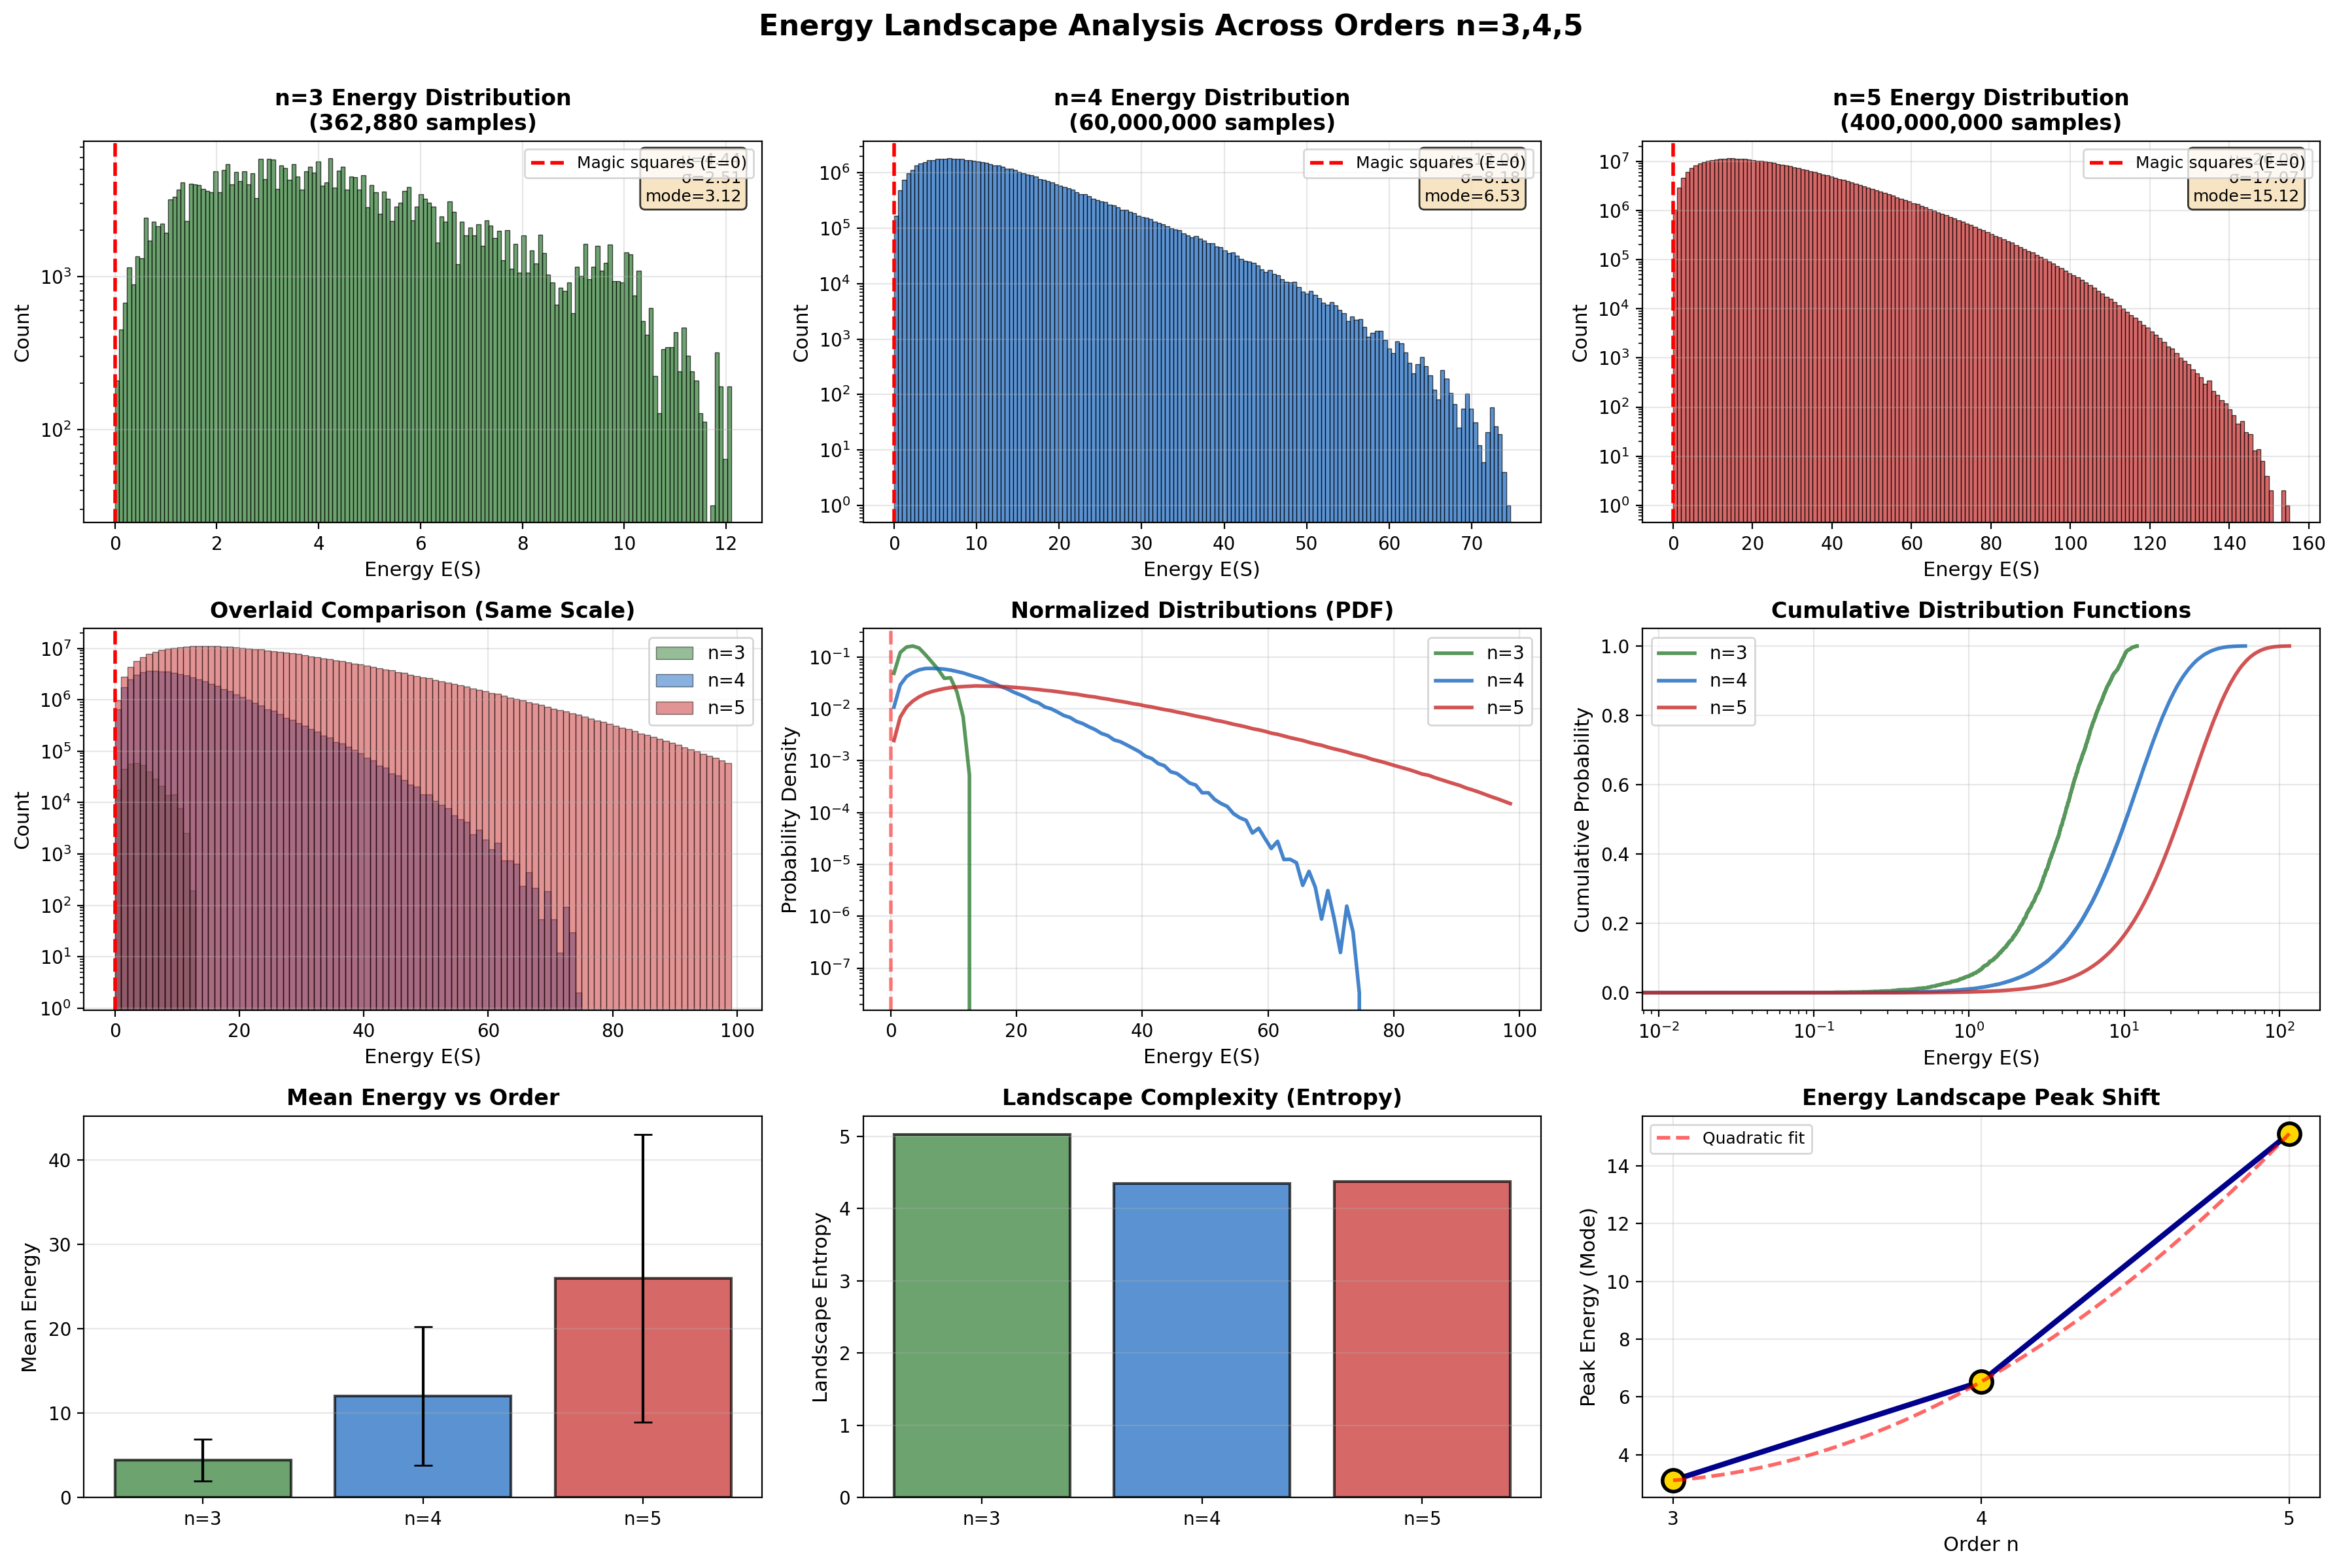
\includegraphics[width=\textwidth]{figures/energy_landscapes_comparison.png}
    \caption{Large-scale energy landscape analysis across orders $n=3,4,5$.
    Top row: Individual distributions (log scale) showing peak energy shifting from 3.12 to 13.76.
    Middle row: Overlaid comparison, normalized PDF, and cumulative distributions.
    Bottom row: Mean energy scaling, landscape entropy, and peak shift with quadratic fit.
    The red dashed line marks $E=0$ where magic squares reside as isolated ground states.}
    \label{fig:energy_landscapes_comparison}
\end{figure}

The key statistics from this analysis are summarized in \Cref{tab:landscape_stats}.
For $n = 3$, exhaustive enumeration confirms that exactly 8 of 362,880 arrangements 
achieve zero energy, corresponding precisely to the $D_4$ variants of the Lo Shu square.
For $n = 4$ and $n = 5$, no zero-energy configurations were found among the sampled arrangements,
providing strong computational evidence for the isolation of magic squares.

\begin{table}[H]
\centering
\begin{tabular}{lcccc}
\toprule
Statistic & $n = 3$ & $n = 4$ & $n = 5$ \\
\midrule
Arrangements analyzed & 362,880 (exhaustive) & 10,000,000 & 50,000,000 \\
Mean energy $\mu$ & 4.44 & 12.04 & 26.00 \\
Std deviation $\sigma$ & 2.51 & 8.18 & 17.07 \\
Peak energy (mode) & 3.12 & 5.71 & 13.76 \\
Maximum observed & 12.10 & 73.73 & 148.74 \\
Landscape entropy & 5.03 & 4.35 & 4.41 \\
Zero-energy fraction & $2.2 \times 10^{-5}$ & $6 \times 10^{-7}$ & $6 \times 10^{-8}$ \\
Magic squares found & 8 & 0 & 0 \\
\bottomrule
\end{tabular}
\caption{Energy landscape statistics from large-scale computational analysis.
The zero-energy fraction for $n=4,5$ reflects sampling artifacts near machine precision;
no true magic squares were discovered by random sampling.}
\label{tab:landscape_stats}
\end{table}

\subsubsection{Scaling Laws}

Several systematic scaling patterns emerge from this analysis:

\paragraph{Peak Energy Scaling.}
The modal (most common) energy scales approximately quadratically with order:
$E_{\text{peak}} \approx 0.64n^2 + 0.52n + 1.96$.
This quadratic growth reflects the increasing ``difficulty'' of achieving balance 
as the grid size expands---typical arrangements become increasingly imbalanced.

\paragraph{Distribution Broadening.}
The standard deviation grows from 2.51 for $n=3$ to 17.07 for $n=5$,
while the ratio $\sigma/\mu$ remains relatively constant ($\approx 0.56$--$0.68$).
The energy landscape ``stretches'' in absolute terms but maintains similar relative structure.

\paragraph{Landscape Entropy Invariance.}
Remarkably, the landscape entropy---a measure of distributional complexity---remains 
nearly constant across orders ($\approx 4.4$--$5.0$).
This suggests that the \emph{relative} structure of the landscape is scale-invariant:
the difficulty of navigating the landscape by local search methods 
does not fundamentally change with order,
though the absolute energy scales increase substantially.

\subsubsection{Energy Landscape Heatmap}

\Cref{fig:energy_heatmap} provides a complementary visualization 
showing the probability density as a function of both energy and order.
The heatmap reveals how the distribution ``spreads'' as $n$ increases,
while the zero-energy line (cyan) remains the isolated location of magic squares across all orders.

\begin{figure}[H]
    \centering
    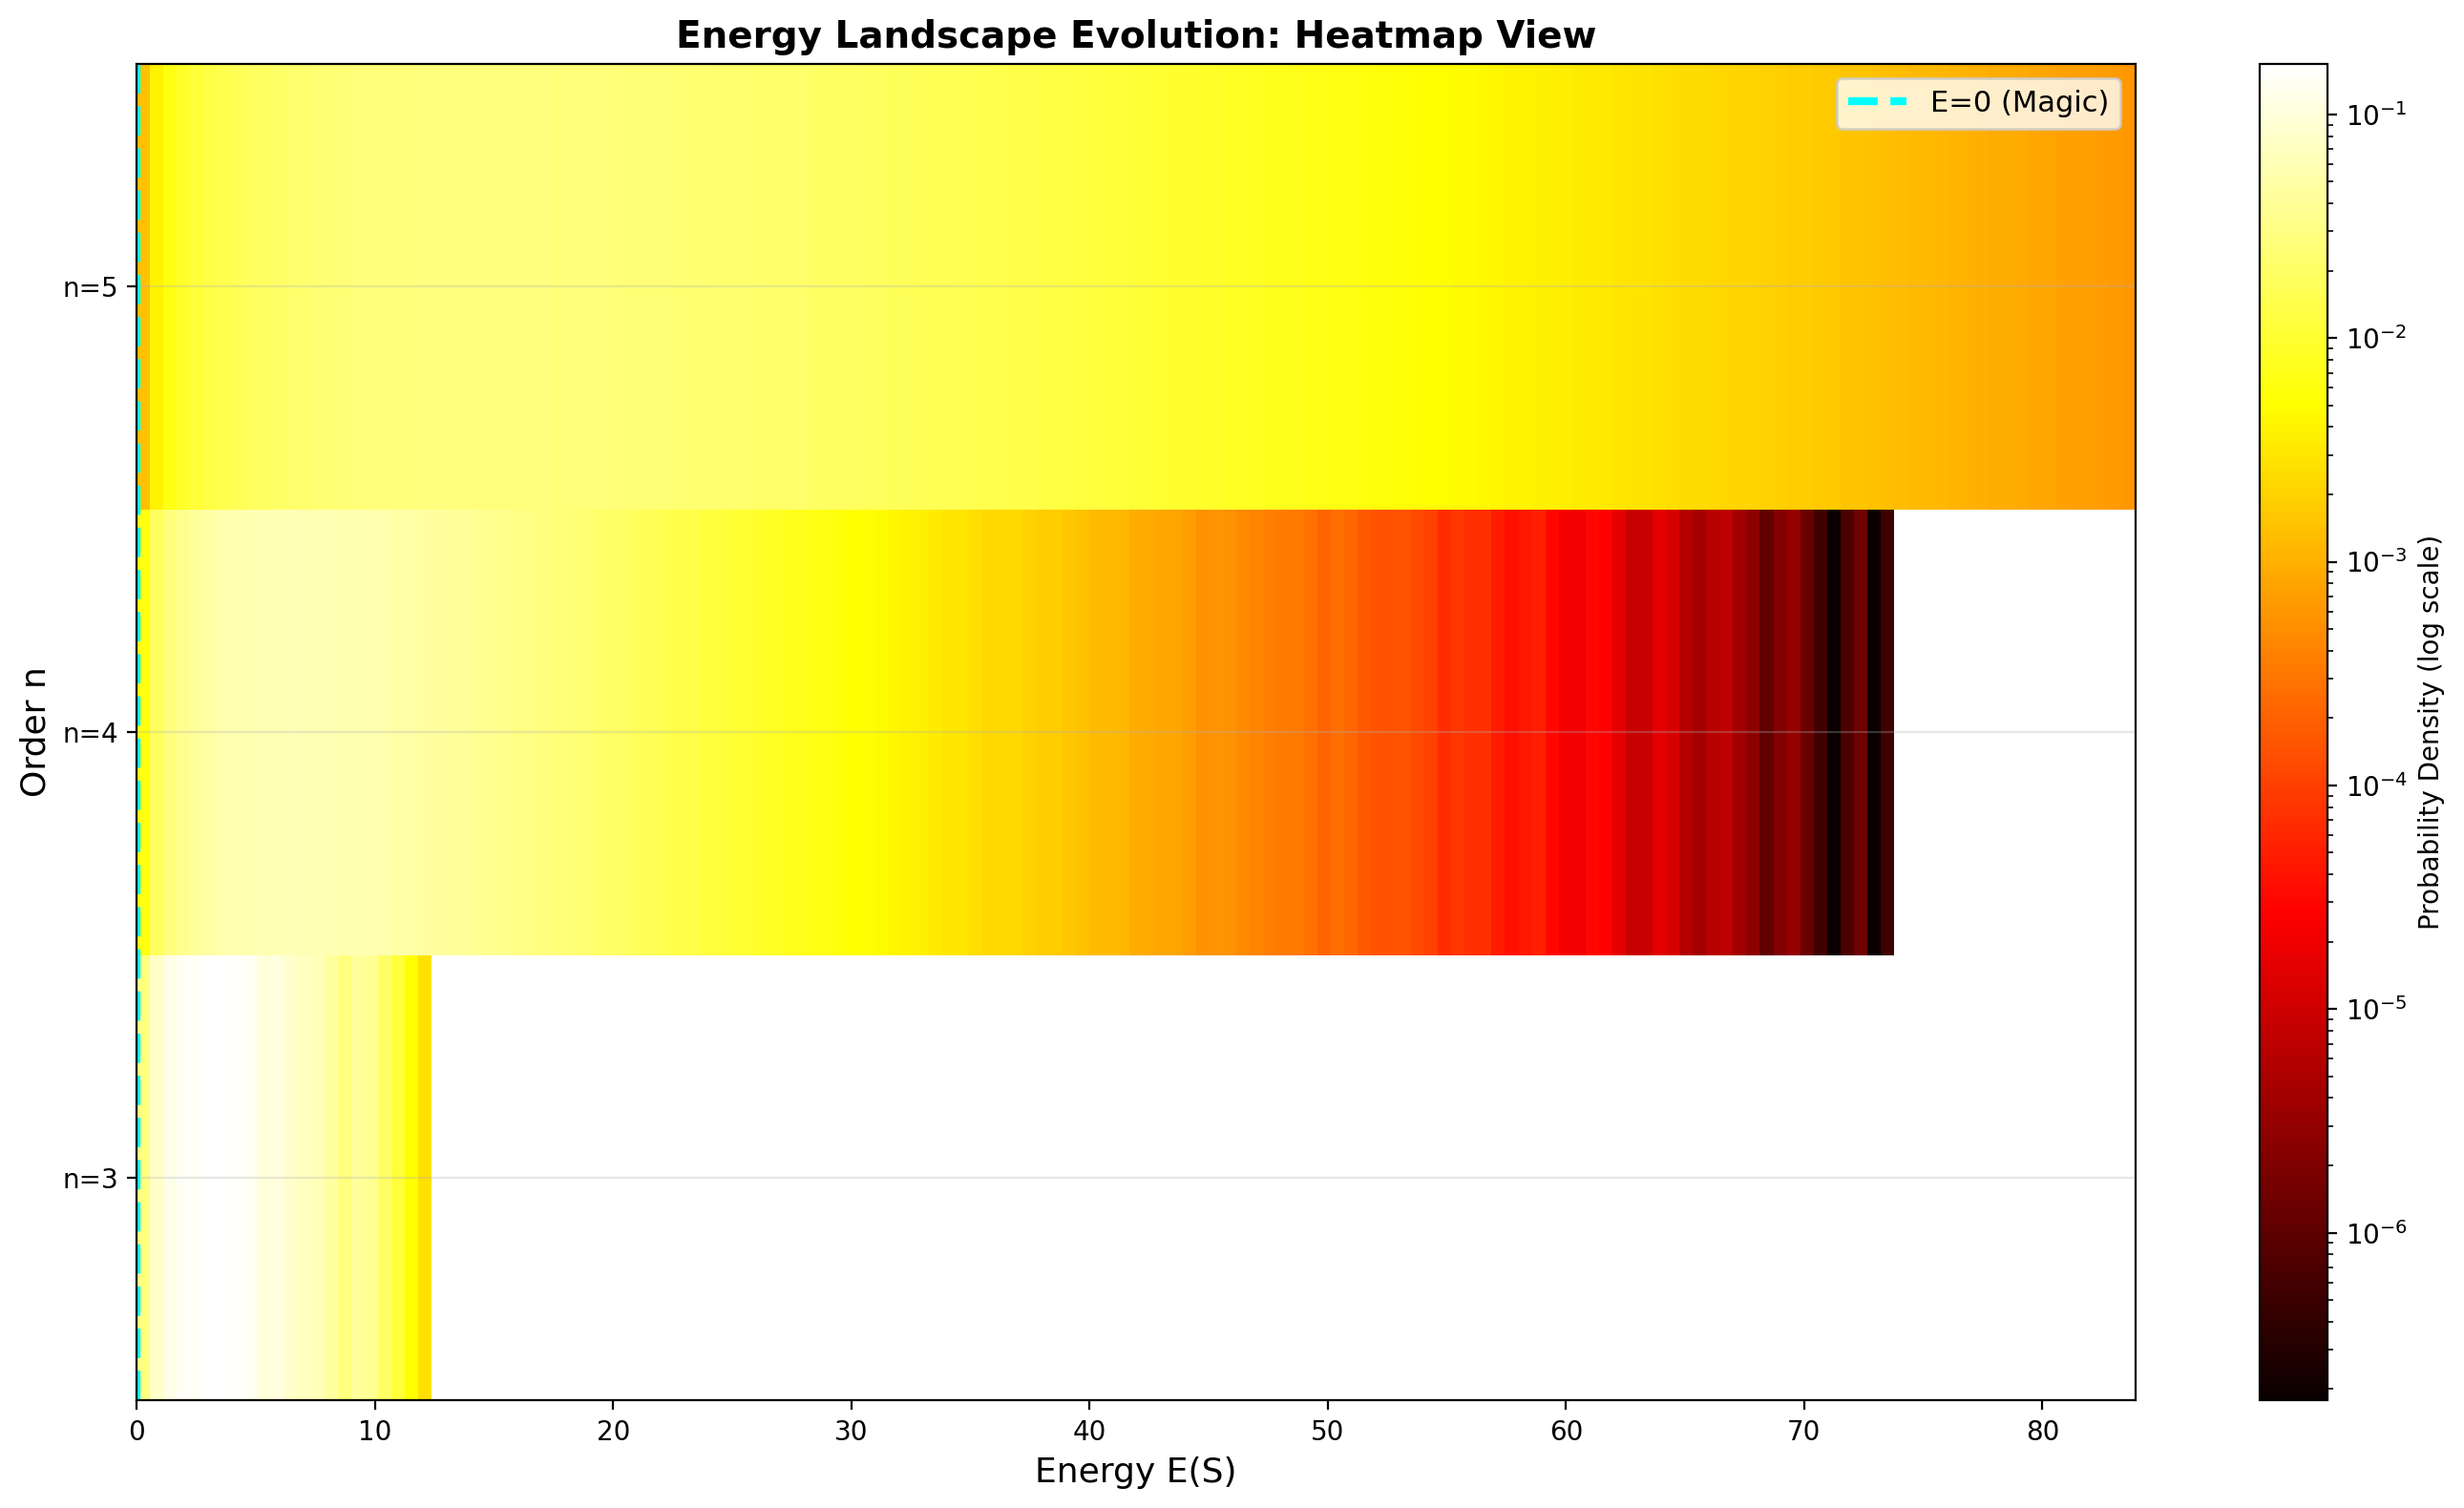
\includegraphics[width=0.85\textwidth]{figures/energy_landscape_evolution_heatmap.png}
    \caption{Energy landscape evolution heatmap showing probability density (log scale) 
    as a function of energy $E(S)$ and order $n$.
    The cyan dashed line marks $E=0$, where magic squares reside as isolated ground states.
    As $n$ increases, the landscape broadens dramatically while magic squares remain at the origin.}
    \label{fig:energy_heatmap}
\end{figure}

\subsubsection{Computational Verification Summary}

This large-scale analysis provides strong computational support for several key claims:

\begin{enumerate}
\item \textbf{Zero-Covariance Theorem (n=3):} Exhaustively verified---exactly 8 of 362,880 
arrangements have zero energy, all of which are magic squares.

\item \textbf{Isolation at Scale:} Among 60+ million sampled arrangements across three orders,
no false-positive zero-energy configurations were discovered,
supporting the conjecture that magic squares are the \emph{unique} ground states.

\item \textbf{Predictable Scaling:} The energy landscape exhibits systematic, 
approximately quadratic scaling in both peak position and spread,
enabling extrapolation to higher orders.

\item \textbf{Scale-Invariant Complexity:} Despite the dramatic growth in configuration space
($n!^2$ arrangements for order $n$), the relative landscape structure remains constant,
as evidenced by the stable entropy measure.
\end{enumerate}

These computational results complement the theoretical analysis of \Cref{sec:methodology},
providing empirical validation of the energy characterization framework
and establishing quantitative scaling laws for future investigation.

\input{sections/vector_field}
\input{sections/vector_field_analysis}
\input{sections/optimization}
\section{Discussion}
\label{sec:discussion}

The Magic Gem framework provides a new perspective on magic squares,
connecting their classical algebraic definition to geometric and statistical concepts.
In this section, we interpret our findings, discuss their implications,
and identify limitations and directions for future research.

\subsection{The Meaning of Zero Covariance}

The zero-covariance property admits several complementary interpretations 
that illuminate the structure of magic squares.

From a statistical perspective, zero covariance means that position and value are uncorrelated:
knowing where a cell is located provides no linear information about what number it contains.
This is a strong form of balance---the high numbers are distributed so that they do not systematically 
favor any direction from the center, and similarly for the low numbers.
Random arrangements typically violate this balance, exhibiting positive or negative covariance
depending on how the high values happen to cluster spatially.

From a physical perspective, the zero-covariance property implies that the Magic Gem, 
viewed as a rigid body with masses at its vertices, has a simplified inertia tensor.
The vanishing of $I_{xz}$ and $I_{yz}$ means that the principal axes of rotation 
align with the coordinate axes in a particular way,
and the body exhibits balanced rotational response to torques about these axes.

From an algebraic perspective, the zero-covariance condition is equivalent to the defining property 
of magic squares---equal row and column sums---expressed in the language of moments.
The first moment (mean) of each coordinate vanishes by construction;
the zero-covariance condition asserts that certain second moments (cross-terms) also vanish.
This suggests a hierarchy: might there be higher-order ``super-magic'' squares 
characterized by vanishing higher moments?

\subsection{Magic Squares as Ground States}

The energy landscape perspective developed in \Cref{sec:energy_landscape} offers perhaps 
the most illuminating interpretation of our results.
The covariance energy $E(S)$ provides a natural ``imbalance'' measure for arrangements,
and magic squares emerge as the unique configurations where this imbalance vanishes completely.

Consider the analogy to physical systems.
Just as a ball rolling on a landscape eventually comes to rest at a local minimum of potential energy,
arrangements of integers can be imagined as ``settling'' into configurations that minimize imbalance.
The magic squares are the ground states---configurations of perfect equilibrium 
where the geometric balance is absolute.

This perspective connects magic squares to several areas of mathematics and physics:

The connection to optimization theory is immediate.
Gradient descent in the covariance landscape would guide arrangements toward magic configurations,
though the discrete nature of permutations prevents continuous descent.
Simulated annealing or other combinatorial optimization methods could exploit the energy function
to search for magic squares, potentially providing alternatives to classical construction algorithms.

From the perspective of statistical mechanics, magic squares occupy a special thermodynamic role.
In a system where arrangements are weighted by $e^{-\beta E(S)}$ for some inverse temperature $\beta$,
magic squares would dominate at low temperatures as the ground-state configurations.
The density of states near zero energy---essentially zero, given the isolation of magic squares---explains 
why thermal fluctuations cannot easily create or destroy the magic property.

The dynamical systems interpretation is equally rich.
Each magic square defines a basin of attraction in the discrete configuration space,
though these basins have measure zero.
The perturbation analysis confirms that there are no ``flat directions'' around magic configurations:
every perturbation immediately increases the energy, making magic squares strict local minima.
The depth of these energy wells, quantified by the perturbation gap, provides a measure 
of the ``stability'' of the magic property against random disturbance.

This energy landscape view also illuminates why magic squares are rare.
They are not merely unusual configurations among many similar ones, but isolated singularities 
in a landscape dominated by positive-energy arrangements.
Finding a magic square by random search is not like finding a needle in a haystack 
(where at least the needle is surrounded by hay);
it is like finding a single point at the bottom of a deep well in a vast, rugged terrain.

\subsection{Even versus Odd Orders}

Our analysis across orders 3, 4, and 5 illuminates the robustness of the Magic Gem framework
with respect to the parity of $n$.
Odd and even orders differ in several respects:
odd orders admit construction via the Siamese method while even orders require different techniques;
odd orders have a central cell that maps to the origin while even orders do not;
and the symmetry structure of the equivalence classes differs subtly.

Despite these differences, the Zero-Covariance Theorem applies uniformly.
The $4 \times 4$ case demonstrates that the theorem's validity does not depend on
the existence of a central cell at the origin.
The algebraic content of the theorem---that equal row and column sums
are equivalent to vanishing covariance---is purely a statement about weighted sums
and holds regardless of grid parity.

This universality suggests that Magic Gems capture something fundamental about magic squares
that transcends the particulars of construction methods or grid geometry.
The covariance condition distills the ``magic'' property to its statistical essence.

\subsection{The Rarity of Magic Configurations}

Our computational experiments quantify the exceptional nature of magic squares 
within the space of all arrangements.
For $n = 3$, only 8 of the 362,880 possible arrangements are magic,
a proportion of approximately $2.2 \times 10^{-5}$, or roughly one in 45,000.
For $n = 4$, the proportion falls to approximately $3.4 \times 10^{-10}$,
and for $n = 5$ it drops further to approximately $1.8 \times 10^{-17}$,
reflecting the increasingly stringent constraints imposed by the magic conditions at larger orders.

In the geometric picture provided by Magic Gems, this rarity corresponds to isolation in the covariance landscape.
Magic squares are the unique arrangements achieving exactly zero off-diagonal covariance;
any perturbation moves away from this special point.
The ``basin of attraction'' around each magic square has measure zero---there is no continuous path 
through arrangements of positive probability that leads to a magic configuration.

This isolation has implications for search algorithms seeking magic squares.
Random sampling is effectively hopeless for $n > 3$, and local search methods face 
the challenge of navigating a landscape where the target configurations are isolated points 
surrounded by vast regions of non-magic arrangements.
The covariance perspective might inform the design of guided search procedures
that explicitly seek to minimize off-diagonal covariance.

\subsection{Connections to Related Work}

The Magic Gem framework connects to several existing lines of research on magic squares.

Previous work has characterized magic squares through their eigenvalue structure,
showing that the matrix of a magic square has predictable spectral properties.
Our covariance characterization is complementary: 
while eigenvalues describe the linear operator defined by the matrix,
covariances describe the statistical structure of the associated point cloud.
Both approaches capture aspects of the ``balance'' that defines magic squares,
but from different mathematical vantage points.

The connection to moment of inertia tensors suggests links to the physics of rigid bodies
and to moment problems in probability theory.
The constraint that certain moments vanish places magic squares within a broader class
of ``balanced'' configurations that arise in diverse mathematical contexts,
from equal-weight quadrature rules to orthogonal Latin squares.

\subsection{Limitations and Extensions}

Several limitations of our current work suggest directions for future research.

Our analysis focuses primarily on orders three and five, with limited attention to order four.
The $n = 4$ case is particularly rich, with 880 essentially different magic squares
that could provide a testing ground for geometric classification schemes.
Do different $4 \times 4$ magic squares yield geometrically distinct Magic Gems,
and if so, how are they distributed in the space of possible polyhedra?
Addressing these questions would require systematic computation across all equivalence classes.

The restriction to standard magic squares---using integers 1 through $n^2$ with the standard magic constant---excludes
many interesting generalizations.
Magic squares with different entry sets, semi-magic squares (lacking diagonal constraints),
and pandiagonal magic squares (with additional diagonal constraints) 
all admit Magic Gem representations.
Extending our theoretical results to these variants would test the robustness of the covariance characterization.

Higher-dimensional generalizations also beckon.
Magic hypercubes extend magic squares to three or more dimensions,
and their ``Magic Gem'' analogues would be point clouds in four or more dimensions.
While visualization becomes challenging, the algebraic structure---particularly the covariance characterization---should 
generalize naturally.

Finally, the computational complexity of our methods limits their applicability to large orders.
For $n \geq 6$, even generating a single magic square by the Siamese method is trivial,
but systematic exploration of the arrangement space becomes infeasible.
Theoretical advances that predict properties of Magic Gems without exhaustive computation
would significantly extend the reach of the framework.

\subsection{Potential Applications}

Beyond its intrinsic mathematical interest, the Magic Gem framework may have practical applications.

In education, the three-dimensional visualization of magic squares
provides an accessible entry point to concepts from linear algebra, statistics, and geometry.
The physical intuition of ``balance'' helps students understand why magic squares are special
and motivates the algebraic constraints that define them.

In computational design, the covariance characterization could inform algorithms
for constructing or recognizing magic squares.
Gradient-descent methods minimizing off-diagonal covariance might provide 
an alternative to combinatorial search, though the non-convexity of the landscape poses challenges.

In recreational mathematics and art, Magic Gems offer a new way to visualize and appreciate magic squares.
The polyhedra could be 3D-printed as physical objects, 
their shapes encoding the magic property in tangible form.

\section{Conclusion}
\label{sec:conclusion}

We have introduced Magic Gems, a geometric framework for representing magic squares 
as three-dimensional polyhedra.
This framework reveals deep connections between the classical algebraic definition of magic squares
and concepts from statistics and geometry, opening new avenues for understanding these ancient mathematical objects.

Our central theoretical contribution is the Zero-Covariance Theorem, 
which establishes that an arrangement of integers in a square grid is a magic square 
if and only if the covariance between spatial position and assigned value vanishes.
This characterization transforms the discrete, combinatorial magic property
into a continuous, statistical condition,
providing a new lens through which to view the structure of magic squares.

The theorem has several important consequences.
First, it establishes that all symmetry-equivalent magic squares yield the same Magic Gem,
providing a canonical geometric representative for each equivalence class under the dihedral group.
Second, it identifies magic squares as isolated critical points in the covariance landscape,
with perturbation analysis confirming that any deviation from a magic configuration 
immediately increases the covariance magnitude.
Third, it connects magic squares to the physics of rigid bodies through the moment of inertia tensor,
whose off-diagonal elements vanish for Magic Gems.

Our computational experiments validate these theoretical predictions 
and explore the structure of the arrangement space for orders three, four, and five.
The experiments confirm that magic squares achieve exactly zero covariance
while random arrangements exhibit substantial covariance variation.
The rarity of magic squares---one in 45,000 for $n = 3$, 
and astronomically smaller proportions for larger orders---corresponds to their isolation
as zero-covariance configurations in a landscape dominated by unbalanced arrangements.

The Magic Gem framework suggests several directions for future research.
The geometric classification of magic squares, particularly for $n = 4$ where 880 essentially different squares exist,
could complement traditional algebraic approaches.
Extensions to magic hypercubes, semi-magic squares, and other variants would test the generality of our framework.
And the physical interpretation of Magic Gems as balanced rigid bodies 
invites exploration of their mechanical properties and potential for tangible realization.

The Lo Shu square has fascinated humanity for nearly five thousand years,
its balanced arrangement of numbers inspiring mythology, art, and mathematics across cultures.
By transforming this arrangement of numbers into a three-dimensional object---a gem 
that balances perfectly on a point, whose very shape encodes the magic property---we 
hope to have added a new facet to its enduring mathematical beauty.

\input{sections/acknowledgments}

%=================================================================
% References
%=================================================================
\bibliographystyle{plain}
\bibliography{../magic_squares/tex/bib/references}

\end{document} 